%% ijbm_SI.tex -- Supplementary material (Appendix A) for ijbm_main.tex,
%% International Journal of Biological Macromolecules format. Text copied from manuscript_short/grip_finding_SI.tex;
%% Sections S12 (methods) and S13 (Table S6) added in the reference cut of 2026-11-24, text moved from the main text.
%% Round 2 (2026-11-24, docs/reviews/2026-11-24_ijbm_editorial_round2.md): sections not cited by the main text removed
%% (ring distortion, waters, pKa, MM/GBSA, rule sections); Table 1 of the main text moved here as Table S1; MD reduced to
%% the three compared systems; new Tables S7 (model), S9 (alpha-amylase-only map); numbers from a44e_round2.py.
\documentclass[preprint,12pt]{elsarticle}
\usepackage{amsmath,amssymb,booktabs,graphicx,longtable,rotating,array}
\usepackage[hidelinks]{hyperref}
\graphicspath{{figures/}}
\renewcommand{\thesection}{S\arabic{section}}
\renewcommand{\thetable}{S\arabic{table}}
\renewcommand{\theequation}{S\arabic{equation}}
\renewcommand{\thefigure}{S\arabic{figure}}
\journal{International Journal of Biological Macromolecules}
\begin{document}
\begin{frontmatter}
\title{Supplementary material for: A fixed core and a variable rim: hydroxyl contacts at the subsites of $\alpha$-amylases and related starch hydrolases, compared with the hydrolysis of substituted starch}
\author[a,b]{Nedis I. Acevedo-Viloria}
\author[c,d]{Yurimar Ruiz-Rocha}
\author[e,d]{Aldo F. Combariza\corref{cor1}}
\ead{aldo.combariza@unisucre.edu.co}
\cortext[cor1]{Corresponding author.}
\affiliation[a]{organization={Programa de Doctorado en Ingenier\'{\i}a, Universidad del Magdalena},
  city={Santa Marta},
  country={Colombia}}
\affiliation[b]{organization={Departamento de Ingenier\'{\i}a Agroindustrial, Facultad de Ingenier\'{\i}as, Universidad de Sucre},
  addressline={Carrera 28 No.\ 5-267},
  city={Sincelejo},
  state={Sucre},
  country={Colombia}}
\affiliation[c]{organization={Departamento de F\'{\i}sica, Facultad de Educaci\'{o}n y Ciencias, Universidad de Sucre},
  addressline={Carrera 28 No.\ 5-267},
  city={Sincelejo},
  state={Sucre},
  country={Colombia}}
\affiliation[d]{organization={Doctorado en Ciencias F\'{\i}sicas, Sistema Universitario Estatal del Caribe (SUE Caribe)},
  country={Colombia}}
\affiliation[e]{organization={Grupo de Investigaci\'{o}n {\itshape in silico},
  Departamento de Biolog\'{\i}a y Qu\'{\i}mica, Facultad de Educaci\'{o}n y Ciencias, Universidad de Sucre},
  addressline={Carrera 28 No.\ 5-267},
  city={Sincelejo},
  state={Sucre},
  country={Colombia}}
\end{frontmatter}

\begin{figure}[h]
\centering
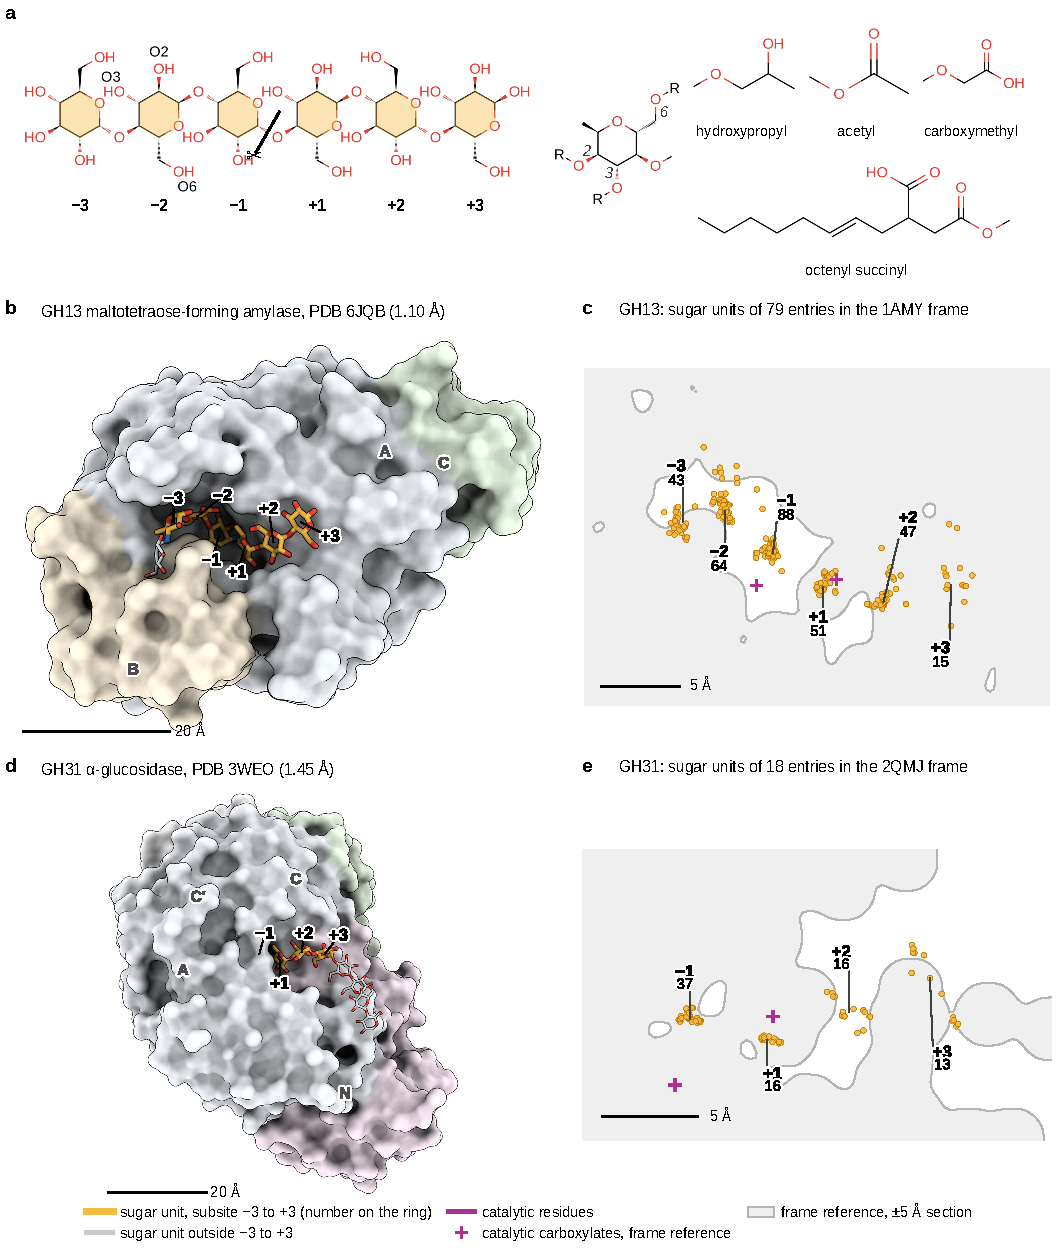
\includegraphics[width=\linewidth]{figS1_protein_surfaces.pdf}
\caption{The structures of Figure~1 of the main text with opaque molecular surfaces. (a) Maltohexaose over
subsites $-3$ to $+3$ with the scissile bond, and the substituents of functionalised starch. (b) GH13
maltotetraose-forming amylase (PDB 6JQB): the cleft is a groove that holds the chain; domains tinted
(B, approximate boundaries). (d) GH31 $\alpha$-glucosidase (PDB 3WEO): subsite $-1$ sits in a pocket. (c, e)
Ring centroids of the sugar units at subsites $-3$ to $+3$ in the family frames, as in Figure~1c,d.}
\label{fig:s1}
\end{figure}

\begin{figure}[h]
\centering
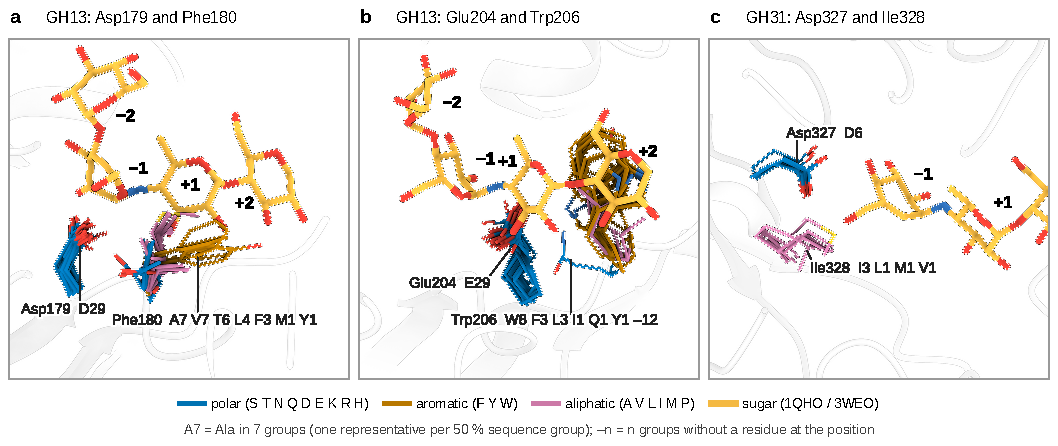
\includegraphics[width=\linewidth]{fig_fixed_variable.pdf}
\caption{Fixed and variable contact positions across 50\% sequence groups, superposed from the best-resolved entry
of every group that has a residue there (a selection of one entry per group, not the full sample): (a) GH13 Asp179
and Phe180, (b) GH13 Glu204 and Trp206, (c) GH31 Asp327 and Ile328 (reference numbering). Side chains coloured by
residue type (blue polar, brown aromatic, pink aliphatic). Labels give the residue types and their number of groups
in one-letter code: D29, Asp in 29 groups; A7, Ala in 7 groups; $-12$, 12 groups without a residue at the position.
Sugar from 1QHO (a, b) or 3WEO (c).}
\label{fig:s2}
\end{figure}


\section{Contact positions of GH13 and GH31 and their conservation}\label{sec:positions}
Table~\ref{tab:positions} lists every reference position of GH13 and GH31 that meets the 20\% contact criterion of
Section~2.2 of the main text, with its class, its residues counted once per 50\% sequence group and its modal fraction
$m$ (eq~1 of the main text). The tests of Table~1 of the main text are computed on these positions.

\begin{table}[p]
\centering\renewcommand{\baselinestretch}{1}\renewcommand{\arraystretch}{0.85}\scriptsize\setlength{\tabcolsep}{3pt}
\caption{Every reference position contacted in at least 20\% of the entries with a sugar unit at subsites $-3$ to
$+3$ (GH13 reference 1AMY, GH31 reference 2QMJ; positions named by the reference residue). Subsites: those at which
the position meets the 20\% criterion; a position is at $-1$/$+1$ when they include $-1$ or $+1$. Class: contact kind
made in most sequence groups (H, side-chain hydrogen bond; Ar, aromatic apolar; Al, aliphatic apolar). Groups:
proteins sharing $\ge$50\% sequence identity that have a residue at the position; residues: votes per group (a mixed
group splits its vote); $m$: modal fraction (eq~1 of the main text); Arom.: aromatic fraction. $^\ast$catalytic residue;
$^\dagger$fewer than five groups. Engineered mutants removed. Class is read from the groups whose residue contacts the
sugar, $m$ over every group with a residue at the position (contacting or not); hence GH13 Phe143 and Gly250 are
classed Ar, from the aromatic residues that make the contact, although Leu (Phe143) or no single residue (Gly250) is
the most common residue over all groups. Source: \texttt{data/analysis/44\_rule\_test/C\_identity\_T20.tsv}.}
\label{tab:positions}
\begin{tabular}{lllrp{4.6cm}rr}
\toprule
Class & Family & Position (subsites) & Groups & Residues (group votes) & $m$ & Arom.\\
\midrule
H & GH13 & Asp179$^\ast$ ($-$1) & 29 & Asp 29 & 1.00 & 0.00\\
H & GH13 & Asp289$^\ast$ ($+$1,$-$1,$-$2) & 28 & Asp 28 & 1.00 & 0.00\\
H & GH13 & Glu204$^\ast$ ($+$1,$-$1) & 29 & Glu 29 & 1.00 & 0.00\\
H & GH13 & His92 ($-$1) & 29 & His 29 & 1.00 & 1.00\\
H & GH13 & Arg177 ($-$1) & 29 & Arg 29 & 1.00 & 0.00\\
H & GH13 & His288 ($-$1) & 29 & His 28, Gln 1 & 0.97 & 0.97\\
H & GH13 & Lys182 ($+$1,$+$2) & 15 & Lys 9.5, Arg 2.5, His 2, Gln 1 & 0.63 & 0.13\\
H & GH13 & Gly183 ($+$1) & 16 & His 8, Gly 5, Tyr 1, Glu 1, Met 1 & 0.50 & 0.56\\
H & GH13 & Gln294 ($-$2) & 15 & Asp 12, Asn 2, Gln 1 & 0.80 & 0.00\\
H & GH13 & Met52 ($-$2,$-$3) & 22 & Asp 9, Trp 5, Asn 3, Gln 2, Gly 2, Phe 1 & 0.41 & 0.27\\
H & GH31 & Asp203 ($+$1) & 5 & Asp 5 & 1.00 & 0.00\\
H & GH31 & Asp327 ($-$1) & 6 & Asp 6 & 1.00 & 0.00\\
H & GH31 & Asp443$^\ast$ ($-$1) & 6 & Asp 6 & 1.00 & 0.00\\
H & GH31 & Asp542$^\ast$ ($+$1,$+$2,$-$1) & 6 & Asp 6 & 1.00 & 0.00\\
H & GH31 & His600 ($-$1) & 6 & His 6 & 1.00 & 1.00\\
H & GH31 & Arg526 ($+$1,$-$1) & 5 & Arg 5 & 1.00 & 0.00\\
H & GH31 & Asn207$^\dagger$ ($+$3) & 2 & His 1, Asn 1 & 0.50 & 0.50\\
\midrule
Ar & GH13 & Tyr51 ($-$1,$-$2) & 29 & Tyr 29 & 1.00 & 1.00\\
Ar & GH13 & Gln49 ($-$2) & 20 & His 11, Trp 6, Val 2, Glu 1 & 0.55 & 0.85\\
Ar & GH13 & Trp206 ($+$1,$+$2,$+$3) & 13 & Trp 7, Phe 3, Ile 1, Tyr 1, Leu 1 & 0.54 & 0.85\\
Ar & GH13 & Phe143 ($-$1) & 21 & Leu 8.5, Phe 7, His 1, Asn 1, Cys 1, Val 1, Ser 1, Tyr 0.5 & 0.41 & 0.41\\
Ar & GH13 & Gly250 ($+$3) & 8 & Tyr 2.5, Phe 2, Thr 1.5, Ser 1, Glu 1 & 0.31 & 0.56\\
Ar & GH31 & Trp406 ($+$1,$-$1) & 5 & Trp 5 & 1.00 & 1.00\\
Ar & GH31 & Trp441 ($-$1) & 6 & Trp 6 & 1.00 & 1.00\\
Ar & GH31 & Phe575 ($+$1,$+$2,$-$1) & 6 & Phe 5, His 1 & 0.83 & 1.00\\
Ar & GH31 & Trp539 ($-$1) & 6 & Trp 5, Phe 1 & 0.83 & 1.00\\
Ar & GH31 & Tyr299 ($+$1,$-$1) & 5 & Tyr 2, Trp 2, Phe 1 & 0.40 & 1.00\\
\midrule
Al & GH13 & Thr207$^\dagger$ ($+$3) & 2 & Lys 2 & 1.00 & 0.00\\
Al & GH13 & Phe180 ($+$1,$-$1) & 29 & Ala 7, Val 7, Thr 6, Leu 4, Phe 3, Tyr 1, Met 1 & 0.24 & 0.14\\
Al & GH31 & Met444 ($+$1,$-$1) & 6 & Met 5, Trp 1 & 0.83 & 0.17\\
Al & GH31 & Ile364 ($-$1) & 6 & Ile 4, Asn 2 & 0.67 & 0.00\\
Al & GH31 & Thr205$^\dagger$ ($+$2,$+$3) & 3 & Ala 2, Pro 1 & 0.67 & 0.00\\
Al & GH31 & Ile328 ($-$1) & 6 & Ile 3, Val 1, Leu 1, Met 1 & 0.50 & 0.00\\
Al & GH31 & Ala576 ($+$2,$+$3) & 5 & Thr 1, Gly 1, Phe 1, Ala 1, Leu 1 & 0.20 & 0.20\\
Al & GH31 & Thr204 ($+$3) & 5 & Asn 1, Asp 1, Gln 1, Ile 1, Leu 1 & 0.20 & 0.00\\
\midrule
none & GH31 & Thr544 ($+$3) & 5 & Ser 1, Lys 1, Thr 1, Ala 1, Trp 1 & 0.20 & 0.20\\
\bottomrule
\end{tabular}
\end{table}

\section{Steric fit of substituents, cell by cell}
Table~\ref{tab:fitcells} gives, for every family $\times$ subsite $\times$ oxygen cell of the map, the
category and the fraction of 50\% sequence groups in which each substituent fits (method in Section~2.5 of
the main text and Section~\ref{sec:sifit}; 3.0~\AA{} flat cut; all glucose-like units). Table~3 of the main text summarises these
categories by state; the table has 70 cells per substituent (O2, O3, deposited O6 and O6$^\ast$), of which Table~3
uses the 52 O2, O3 and O6$^\ast$ cells with a state. The screen measures free volume in the deposited coordinates only. The fit categories are F, fits in at least half of the groups; s, fits in at least
one unit but in fewer than half of the groups; N, fits in no unit. Results at 2.8 and 3.2~\AA, with the
polar-aware rule, for glucose units only, per entry and per unit are in
\texttt{data/analysis/46\_substituent\_fit/} (\texttt{cell\_fit\_summary.tsv}, \texttt{site\_results.tsv},
\texttt{REPORT.md}).

Against the 36 cell--substituent pairs with a literature result, the screen agrees cleanly in 16 (tolerated with F,
not tolerated with N), partially in 15 (s, or a mixed verdict in the literature) and disagrees in 5. Phosphate on O6
at $+1$ of GH15 and of GH14 is tolerated by the enzymes but fits in no pose (glucoamylase Trp52; best
$\beta$-amylase clearance 2.1--2.5~\AA; the GH15 O6 is modelled, and the GH14 structures are soybean and
\emph{Bacillus cereus}, not sweet-potato, $\beta$-amylase). Methyl on O6 at $-1$ of GH15 and on O2 at $-1$ of GH14 is
not tolerated yet fits, at oxygens that are hydrogen-bonded (INV and MC); the screen does not count the hydrogen bond
lost when the hydroxyl hydrogen is replaced. Methyl on O6 at $+1$ of GH13 fits in 17 of 17 groups while the terminal
residues of \emph{B.~subtilis} limit dextrins are $>$90\% unsubstituted~\citep{vanderBurgt2000b}, a result that does
not resolve the position of the methyl group. The limits: protein and chain are static, the conformers carry no
energies, inhibitor units dominate $-1$ and $+1$, O6 at $+1$ in GH31 and GH15 is tested only on modelled rotamers,
GH14 and GH15 rest on two groups each, and symmetry mates were not generated.

{\scriptsize\setlength{\tabcolsep}{3pt}
\begin{longtable}{llllrrllllllll}
\caption{Fit category and fraction of 50\% sequence groups in which the substituent fits, per cell
(3.0~\AA{} flat cut, all glucose-like units). State: the cell state of the map (main text,
Section~2.4); O6, deposited O6; O6$^\ast$, deposited O6 or any of the gg, gt, tg rotamers (for O6$^\ast$
the state shown is that of the deposited O6; --, no O6 deposited). Groups and units: numbers of 50\%
sequence groups and of units in the cell. Me, methyl; HE, 2-hydroxyethyl; HP, 2-hydroxypropyl; Ac,
acetyl; CM, carboxymethyl; P, phosphate; Suc, succinyl; OSA, octenylsuccinyl. Source:
\texttt{data/analysis/46\_substituent\_fit/cell\_fit\_summary.tsv}.}\label{tab:fitcells}\\
\toprule
Fam. & Sub. & O & State & Groups & Units & Me & HE & HP & Ac & CM & P & Suc & OSA\\
\midrule
\endfirsthead
\toprule
Fam. & Sub. & O & State & Groups & Units & Me & HE & HP & Ac & CM & P & Suc & OSA\\
\midrule
\endhead
\bottomrule
\endfoot
GH13 & $-$3 & O2 & EXP & 17 & 43 & F\,0.82 & F\,0.77 & F\,0.77 & F\,0.71 & F\,0.71 & s\,0.29 & F\,0.65 & F\,0.65\\
GH13 & $-$3 & O3 & EXP & 17 & 43 & F\,0.88 & F\,0.88 & F\,0.88 & F\,0.82 & F\,0.82 & s\,0.47 & F\,0.88 & F\,0.88\\
GH13 & $-$3 & O6 & EXP & 10 & 24 & F\,1.00 & F\,1.00 & F\,1.00 & F\,1.00 & F\,1.00 & F\,0.60 & F\,0.90 & F\,0.80\\
GH13 & $-$3 & O6$^\ast$ & EXP & 17 & 43 & F\,0.88 & F\,0.88 & F\,0.88 & F\,0.88 & F\,0.88 & F\,0.53 & F\,0.82 & F\,0.82\\
GH13 & $-$2 & O2 & VAR & 22 & 63 & s\,0.36 & s\,0.27 & s\,0.04 & s\,0.04 & s\,0.09 & N\,0.00 & s\,0.00 & s\,0.00\\
GH13 & $-$2 & O3 & VAR & 22 & 63 & F\,0.73 & F\,0.64 & F\,0.50 & s\,0.46 & s\,0.41 & s\,0.09 & s\,0.27 & s\,0.27\\
GH13 & $-$2 & O6 & VAR & 21 & 61 & F\,0.67 & s\,0.38 & s\,0.29 & s\,0.14 & s\,0.29 & s\,0.00 & s\,0.14 & s\,0.14\\
GH13 & $-$2 & O6$^\ast$ & VAR & 22 & 63 & F\,0.86 & F\,0.64 & F\,0.59 & s\,0.41 & F\,0.59 & s\,0.09 & s\,0.41 & s\,0.36\\
GH13 & $-$1 & O2 & INV & 29 & 82 & s\,0.03 & s\,0.00 & s\,0.00 & N\,0.00 & s\,0.00 & N\,0.00 & N\,0.00 & N\,0.00\\
GH13 & $-$1 & O3 & INV & 29 & 82 & s\,0.00 & s\,0.00 & s\,0.00 & N\,0.00 & N\,0.00 & N\,0.00 & N\,0.00 & N\,0.00\\
GH13 & $-$1 & O6 & INV & 29 & 82 & s\,0.03 & s\,0.03 & s\,0.03 & s\,0.03 & s\,0.03 & N\,0.00 & s\,0.03 & N\,0.00\\
GH13 & $-$1 & O6$^\ast$ & INV & 29 & 82 & s\,0.48 & s\,0.28 & s\,0.17 & s\,0.07 & s\,0.14 & N\,0.00 & s\,0.03 & N\,0.00\\
GH13 & $+$1 & O2 & VAR & 17 & 50 & s\,0.35 & s\,0.06 & N\,0.00 & s\,0.06 & N\,0.00 & N\,0.00 & N\,0.00 & N\,0.00\\
GH13 & $+$1 & O3 & INV & 17 & 50 & s\,0.06 & s\,0.06 & N\,0.00 & N\,0.00 & N\,0.00 & N\,0.00 & N\,0.00 & N\,0.00\\
GH13 & $+$1 & O6 & BUR & 3 & 3 & s\,0.33 & s\,0.33 & s\,0.33 & s\,0.33 & s\,0.33 & s\,0.33 & s\,0.33 & s\,0.33\\
GH13 & $+$1 & O6$^\ast$ & BUR & 17 & 50 & F\,1.00 & F\,0.88 & F\,0.71 & F\,0.77 & F\,0.71 & F\,0.53 & F\,0.59 & F\,0.53\\
GH13 & $+$2 & O2 & VAR & 15 & 47 & F\,0.80 & F\,0.60 & F\,0.60 & F\,0.53 & s\,0.47 & s\,0.20 & F\,0.53 & s\,0.47\\
GH13 & $+$2 & O3 & VAR & 15 & 47 & s\,0.47 & s\,0.40 & s\,0.27 & s\,0.13 & s\,0.20 & N\,0.00 & s\,0.07 & s\,0.07\\
GH13 & $+$2 & O6 & EXP & 15 & 47 & F\,0.93 & F\,0.87 & F\,0.87 & F\,0.80 & F\,0.87 & F\,0.60 & F\,0.80 & F\,0.73\\
GH13 & $+$2 & O6$^\ast$ & EXP & 15 & 47 & F\,1.00 & F\,0.93 & F\,0.93 & F\,0.93 & F\,0.93 & F\,0.67 & F\,0.93 & F\,0.87\\
GH13 & $+$3 & O2 & MC & 10 & 14 & F\,1.00 & F\,1.00 & F\,1.00 & F\,0.50 & F\,1.00 & s\,0.40 & F\,0.50 & s\,0.40\\
GH13 & $+$3 & O3 & MC & 10 & 14 & F\,1.00 & F\,0.90 & F\,0.80 & F\,0.60 & F\,0.50 & s\,0.20 & s\,0.40 & s\,0.40\\
GH13 & $+$3 & O6 & EXP & 10 & 14 & F\,1.00 & F\,1.00 & F\,0.80 & F\,0.70 & F\,0.80 & F\,0.50 & F\,0.70 & F\,0.70\\
GH13 & $+$3 & O6$^\ast$ & EXP & 10 & 14 & F\,1.00 & F\,1.00 & F\,0.80 & F\,0.80 & F\,0.80 & F\,0.60 & F\,0.80 & F\,0.80\\
\addlinespace
GH31 & $-$1 & O2 & INV & 6 & 32 & s\,0.00 & N\,0.00 & N\,0.00 & N\,0.00 & N\,0.00 & N\,0.00 & N\,0.00 & N\,0.00\\
GH31 & $-$1 & O3 & INV & 6 & 32 & F\,1.00 & N\,0.00 & N\,0.00 & N\,0.00 & N\,0.00 & N\,0.00 & N\,0.00 & N\,0.00\\
GH31 & $-$1 & O6 & INV & 6 & 32 & F\,0.50 & N\,0.00 & N\,0.00 & N\,0.00 & N\,0.00 & N\,0.00 & N\,0.00 & N\,0.00\\
GH31 & $-$1 & O6$^\ast$ & INV & 6 & 32 & F\,0.67 & N\,0.00 & N\,0.00 & N\,0.00 & N\,0.00 & N\,0.00 & N\,0.00 & N\,0.00\\
GH31 & $+$1 & O2 & INV & 5 & 16 & F\,0.60 & F\,0.60 & s\,0.40 & s\,0.40 & F\,0.60 & N\,0.00 & s\,0.20 & N\,0.00\\
GH31 & $+$1 & O3 & INV & 5 & 16 & N\,0.00 & N\,0.00 & N\,0.00 & N\,0.00 & N\,0.00 & N\,0.00 & N\,0.00 & N\,0.00\\
GH31 & $+$1 & O6$^\ast$ & -- & 5 & 16 & F\,1.00 & F\,0.60 & F\,0.60 & s\,0.20 & s\,0.20 & N\,0.00 & N\,0.00 & N\,0.00\\
GH31 & $+$2 & O2 & EXP & 5 & 16 & F\,1.00 & F\,1.00 & F\,0.80 & F\,0.60 & F\,0.80 & F\,0.60 & F\,0.60 & s\,0.40\\
GH31 & $+$2 & O3 & EXP & 5 & 16 & F\,1.00 & F\,0.80 & F\,0.80 & F\,0.80 & F\,0.80 & s\,0.00 & s\,0.40 & s\,0.40\\
GH31 & $+$2 & O6 & EXP & 5 & 16 & F\,1.00 & F\,0.80 & F\,0.80 & s\,0.40 & F\,0.80 & s\,0.20 & s\,0.40 & s\,0.20\\
GH31 & $+$2 & O6$^\ast$ & EXP & 5 & 16 & F\,1.00 & F\,0.80 & F\,0.80 & s\,0.40 & F\,0.80 & s\,0.20 & s\,0.40 & s\,0.20\\
GH31 & $+$3 & O2 & EXP & 5 & 13 & F\,1.00 & F\,1.00 & F\,1.00 & F\,1.00 & F\,0.80 & F\,0.60 & F\,1.00 & F\,1.00\\
GH31 & $+$3 & O3 & EXP & 5 & 13 & F\,1.00 & F\,1.00 & F\,1.00 & F\,1.00 & F\,1.00 & F\,0.80 & F\,1.00 & F\,1.00\\
GH31 & $+$3 & O6 & BUR & 5 & 13 & F\,1.00 & F\,1.00 & F\,1.00 & s\,0.20 & F\,0.80 & s\,0.20 & s\,0.20 & s\,0.20\\
GH31 & $+$3 & O6$^\ast$ & BUR & 5 & 13 & F\,1.00 & F\,1.00 & F\,1.00 & F\,0.80 & F\,1.00 & s\,0.20 & F\,0.60 & F\,0.60\\
\addlinespace
GH14 & $-$2 & O2 & VAR & 2 & 18 & s\,0.00 & s\,0.00 & s\,0.00 & s\,0.00 & s\,0.00 & s\,0.00 & s\,0.00 & s\,0.00\\
GH14 & $-$2 & O3 & INV & 2 & 18 & F\,1.00 & N\,0.00 & N\,0.00 & N\,0.00 & N\,0.00 & N\,0.00 & N\,0.00 & N\,0.00\\
GH14 & $-$2 & O6 & INV & 2 & 18 & N\,0.00 & N\,0.00 & N\,0.00 & N\,0.00 & N\,0.00 & N\,0.00 & N\,0.00 & N\,0.00\\
GH14 & $-$2 & O6$^\ast$ & INV & 2 & 18 & N\,0.00 & N\,0.00 & N\,0.00 & N\,0.00 & N\,0.00 & N\,0.00 & N\,0.00 & N\,0.00\\
GH14 & $-$1 & O2 & MC & 2 & 19 & F\,1.00 & F\,1.00 & F\,1.00 & F\,0.50 & F\,0.50 & F\,0.50 & F\,0.50 & s\,0.00\\
GH14 & $-$1 & O3 & MC & 2 & 18 & s\,0.00 & s\,0.00 & s\,0.00 & s\,0.00 & s\,0.00 & s\,0.00 & s\,0.00 & s\,0.00\\
GH14 & $-$1 & O6 & INV & 2 & 19 & s\,0.00 & N\,0.00 & N\,0.00 & N\,0.00 & N\,0.00 & N\,0.00 & N\,0.00 & N\,0.00\\
GH14 & $-$1 & O6$^\ast$ & INV & 2 & 19 & s\,0.00 & s\,0.00 & N\,0.00 & N\,0.00 & N\,0.00 & N\,0.00 & N\,0.00 & N\,0.00\\
GH14 & $+$1 & O2 & MC & 2 & 3 & N\,0.00 & N\,0.00 & N\,0.00 & N\,0.00 & N\,0.00 & N\,0.00 & N\,0.00 & N\,0.00\\
GH14 & $+$1 & O3 & INV & 2 & 3 & N\,0.00 & N\,0.00 & N\,0.00 & N\,0.00 & N\,0.00 & N\,0.00 & N\,0.00 & N\,0.00\\
GH14 & $+$1 & O6 & INV & 2 & 3 & F\,0.50 & F\,0.50 & N\,0.00 & N\,0.00 & N\,0.00 & N\,0.00 & N\,0.00 & N\,0.00\\
GH14 & $+$1 & O6$^\ast$ & INV & 2 & 3 & F\,1.00 & F\,1.00 & F\,0.50 & N\,0.00 & F\,0.50 & N\,0.00 & N\,0.00 & N\,0.00\\
GH14 & $+$2 & O2 & INV & 2 & 3 & F\,1.00 & F\,1.00 & F\,0.50 & N\,0.00 & F\,0.50 & N\,0.00 & N\,0.00 & N\,0.00\\
GH14 & $+$2 & O3 & INV & 2 & 3 & N\,0.00 & N\,0.00 & N\,0.00 & N\,0.00 & N\,0.00 & N\,0.00 & N\,0.00 & N\,0.00\\
GH14 & $+$2 & O6 & BUR & 2 & 3 & F\,1.00 & F\,1.00 & F\,0.50 & N\,0.00 & F\,0.50 & N\,0.00 & N\,0.00 & N\,0.00\\
GH14 & $+$2 & O6$^\ast$ & BUR & 2 & 3 & F\,1.00 & F\,1.00 & F\,0.50 & F\,0.50 & F\,0.50 & N\,0.00 & F\,0.50 & F\,0.50\\
\addlinespace
GH15 & $-$1 & O2 & INV & 2 & 5 & N\,0.00 & N\,0.00 & N\,0.00 & N\,0.00 & N\,0.00 & N\,0.00 & N\,0.00 & N\,0.00\\
GH15 & $-$1 & O3 & INV & 2 & 5 & s\,0.00 & N\,0.00 & N\,0.00 & N\,0.00 & N\,0.00 & N\,0.00 & N\,0.00 & N\,0.00\\
GH15 & $-$1 & O6 & INV & 2 & 5 & F\,1.00 & N\,0.00 & N\,0.00 & N\,0.00 & N\,0.00 & N\,0.00 & N\,0.00 & N\,0.00\\
GH15 & $-$1 & O6$^\ast$ & INV & 2 & 5 & F\,1.00 & N\,0.00 & N\,0.00 & N\,0.00 & N\,0.00 & N\,0.00 & N\,0.00 & N\,0.00\\
GH15 & $+$1 & O2 & INV & 2 & 5 & F\,1.00 & F\,1.00 & F\,1.00 & F\,1.00 & F\,1.00 & N\,0.00 & F\,1.00 & F\,1.00\\
GH15 & $+$1 & O3 & INV & 2 & 5 & N\,0.00 & N\,0.00 & N\,0.00 & N\,0.00 & N\,0.00 & N\,0.00 & N\,0.00 & N\,0.00\\
GH15 & $+$1 & O6$^\ast$ & -- & 2 & 5 & F\,1.00 & F\,1.00 & F\,0.50 & N\,0.00 & N\,0.00 & N\,0.00 & N\,0.00 & N\,0.00\\
GH15 & $+$2 & O2 & EXP & 2 & 5 & F\,1.00 & F\,1.00 & F\,1.00 & F\,1.00 & F\,1.00 & F\,0.50 & F\,1.00 & F\,1.00\\
GH15 & $+$2 & O3 & EXP & 2 & 5 & F\,1.00 & F\,1.00 & F\,1.00 & F\,1.00 & F\,1.00 & F\,0.50 & F\,1.00 & F\,1.00\\
GH15 & $+$2 & O6 & MC & 2 & 5 & N\,0.00 & N\,0.00 & N\,0.00 & N\,0.00 & N\,0.00 & N\,0.00 & N\,0.00 & N\,0.00\\
GH15 & $+$2 & O6$^\ast$ & MC & 2 & 5 & N\,0.00 & N\,0.00 & N\,0.00 & N\,0.00 & N\,0.00 & N\,0.00 & N\,0.00 & N\,0.00\\
GH15 & $+$3 & O2 & EXP & 2 & 5 & F\,1.00 & F\,1.00 & F\,1.00 & F\,1.00 & F\,1.00 & F\,1.00 & F\,1.00 & F\,1.00\\
GH15 & $+$3 & O3 & EXP & 2 & 5 & F\,1.00 & F\,1.00 & F\,1.00 & F\,0.50 & F\,1.00 & F\,0.50 & F\,1.00 & F\,1.00\\
GH15 & $+$3 & O6 & EXP & 2 & 5 & F\,1.00 & F\,1.00 & F\,1.00 & F\,0.50 & F\,1.00 & s\,0.00 & F\,0.50 & F\,0.50\\
GH15 & $+$3 & O6$^\ast$ & EXP & 2 & 5 & F\,1.00 & F\,1.00 & F\,1.00 & F\,0.50 & F\,1.00 & s\,0.00 & F\,0.50 & F\,0.50\\
\end{longtable}}

\section{Molecular dynamics of three glucose-only complexes}\label{sec:md}
At $-1$ and $+1$ the crystal map rests mostly on inhibitor rings, and the $+1$ ring of acarbose has no O6. Wild-type
complexes with a glucose-only glucan at the catalytic subsites were simulated (method in Section~\ref{sec:simd}) to see
whether unmodified glucose units in a moving protein keep the crystal states. Three complexes of families with a
crystal map qualify and are compared here (Table~\ref{tab:mdsys}): 7DCG and 6A0K (GH13) and 1J18 (GH14); GH31 and
GH15 have no wild-type glucose-only complex. The runs are unfinished: one replica each, analysed at 21.8, 22.9 and
23.5 of 100~ns (219, 230 and 236 frames read every 100~ps). No equilibration or convergence analysis was made beyond
comparing the first and second halves of each trajectory, and the results are not used in the main text.

In GH13 at $-1$, the 11 cells of the two $-1$ units (O1--O6 of 6A0K, O2--O6 of 7DCG) all keep the crystal-map
state: O2 and O3 are held by fixed residues in 100\% of frames and O6 in 91\% (7DCG) and 94\% (6A0K). At $+1$
(7DCG only), O3 is held by Glu204 in 99.5\% of frames, as in the map, whereas O6, which the crystal map has as buried
from three units, is free and exposed (held in 3\% of frames, median 15.4~\AA$^2$ open). The scissile O4 of the $+1$
unit, held by catalytic residues in every crystal group (INV), is held in 37\% of the 7DCG frames (Glu204 31\%, Asp289
8\%; 48\% in the first half of the run and 26\% in the second) and in 11\% of the 1J18 frames (Glu186): the
simulations do not reproduce that cell. In GH14 (1J18), O6 at $+1$ is held in 82\% of frames by Glu186, Arg188 and
Tyr192, as in the crystal map, so the disagreement of that cell with the sweet-potato $\beta$-amylase result
(Table~\ref{tab:mapexp}) remains. Over the 48 cells of the three complexes that have a crystal state, 35 keep the
state and 40 keep the distinction between held and not held. Sources:
\texttt{data/analysis/47\_md\_hydroxyl/md\_cells.tsv},
\texttt{data/analysis/44\_rule\_test/revision2/E\_md\_three\_systems.tsv}.

\begin{table}[h]
\centering\scriptsize\setlength{\tabcolsep}{3pt}
\caption{The three simulated complexes compared with the crystal map. ns, frames: length of trajectory analysed, read
every 100~ps, out of 100~ns. Sources: \texttt{data/calc/08\_md/selection/selection.tsv},
\texttt{data/analysis/47\_md\_hydroxyl/systems.tsv}.}
\label{tab:mdsys}
\begin{tabular}{llp{4.2cm}rp{3.4cm}rr}
\toprule
PDB & Family & Enzyme & Res. (\AA) & Glucan & ns & Frames\\
\midrule
7DCG & GH13 & \emph{Weissella cibaria} $\alpha$-glucosidase & 1.53 & maltotriose & 21.8 & 219\\
6A0K & GH13 & \emph{Arthrobacter globiformis} cyclic maltosyl-maltose hydrolase & 1.94 & trisaccharide, one $\alpha(1\!\to\!4)$ and one $\alpha(1\!\to\!6)$ linkage & 22.9 & 230\\
1J18 & GH14 & \emph{Bacillus cereus} $\beta$-amylase & 2.00 & maltotetraose & 23.5 & 236\\
\bottomrule
\end{tabular}
\end{table}

\section{GH14 and GH15: two sequence groups each}\label{sec:gh1415}
GH14 ($\beta$-amylase, an inverting enzyme in no clan) and GH15 (glucoamylase, an inverting $(\alpha/\alpha)_6$ fold)
enter the map of the main text but not the residue test, because each has only two 50\% sequence groups among its
ligand-bound entries (GH14: barley and soybean, 66\% identical, and \emph{Bacillus cereus}, about 30\% to both; GH15:
three proteins, two fungal glucoamylases 34\% identical and a third whose UniProt accession, Q12537, could not be
resolved). Counted per entry, the GH14 side chains that hydrogen-bond the sugar at $-1$ and $-2$ (Asp53, His93,
Arg420, the base Glu380, Lys295, the acid Glu186) and the aromatic Trp55 are the same residue in every entry that
contacts them (Glu186 is contacted in 14 entries and hydrogen-bonds the sugar in 10). In GH15 the hydrogen-bonding
side chains (Asp55, Arg54, the acid Glu179, Glu180, Arg305) and six aromatic residues (Tyr48, Trp52, Trp317, Trp417,
Trp120, Tyr311) are the same over four entries. The aliphatic residues of both families (GH14 Leu419, Leu20, Met17,
Ala184; GH15 Leu177, Leu415, Ala39) are also the same. With two groups no residue can be shown to vary, so the
comparison between kinds of contact made for GH13 and GH31 cannot be made in these families, and an ``invariant''
partner in their map (Section~2.4 of the main text) is one conserved in both groups. Positions are named in the
numbering of soybean $\beta$-amylase (1BYA~\citep{Mikami1994}) and \emph{Aspergillus awamori} glucoamylase
(1AGM~\citep{Aleshin1994}).

\section{Supplementary methods}\label{sec:simethods}
The settings of the open-surface and free-volume calculations (main text, Sections 2.4 and 2.5) and of the
molecular dynamics of Section~\ref{sec:md} are given here in full.

\subsection{Open surface of the glucose oxygens}\label{sec:sisasa}
The open surface of each glucose oxygen (main text, Section~2.4) was computed by the Shrake--Rupley
method~\citep{Shrake1973} (480 points per atom, probe 1.4~\AA, Bondi radii, no hydrogens, waters removed) in
the complex and in the ligand alone.

\subsection{Free volume around the oxygens (steric fit of substituents)}\label{sec:sifit}
The 439 units of Section~2.4 of the main text were used with the deposited protein and sugar fixed.
Eight substituents were built as fragments Cprev--\allowbreak Cring--\allowbreak O--\allowbreak R with RDKit 2025.03 (ETKDGv3
conformers~\citep{Wang2020}, each optimised with MMFF94~\citep{Halgren1996}, hydrogens then removed): methyl, 2-\hspace{0pt}hydroxyethyl,
2-\hspace{0pt}hydroxypropyl (both configurations), acetyl, carboxymethyl, phosphate monoester,
succinyl and octenylsuccinyl (both configurations at the branch carbon, $E$ alkene); 9 to 400 conformers
per substituent and configuration. Each conformer was placed on the deposited Cprev, Cring and O of O2, O3 and O6 (the
deposited oxygen becomes the attachment oxygen) and turned about the Cring--O bond in 30$^\circ$ steps
(108 to 9\,600 poses per site). O6 was tested at its deposited position and rebuilt at the gg, gt and
tg rotamers ($\omega = -60^\circ$, $+60^\circ$, $180^\circ$); O6$^\ast$ means a fit at any of the four,
the only test possible where no O6 is deposited. A pose fits when no substituent heavy atom lies within
3.0~\AA{} of a protein heavy atom of the asymmetric unit or within 2.8~\AA{} of another sugar atom (atoms
within three bonds excluded); 2.8 and 3.2~\AA{}, and a polar-aware rule that lets a substituent O/N
approach a protein N/O to 2.5~\AA, were run as sensitivity tests. A unit fits when any pose fits, and
the counting goes from unit to entry to 50\% sequence group as in Section~2.4 of the main text. A cell
is F when the substituent fits in at least half of the groups, s when it fits in at least one unit
but in fewer than half of the groups, and N when it fits in no unit. The one assumption is that the
deposited coordinates are where a substituted chain would sit.

\subsection{Molecular dynamics of enzyme--glucan complexes}\label{sec:simd}
Wild-type complexes with a glucose-only glucan of 2--7 units (every unit RSCC $\ge0.80$, X-ray at
$\le2.2$~\AA, no mutation, not cyclic, no covalent bond to another molecule) were selected; 83 glucans of 42 entries
passed, in AA13, GH13, GH14, GH49, GH57 and GT35. Twelve complexes were simulated, one per family and in GH13 one per
enzyme type; the three of Table~\ref{tab:mdsys} are those with the glucan at the catalytic subsites of a family with a
crystal map (the others have the glucan at secondary sites, or are of GH57, which has no map, and are not used). The protein was described by
ff14SB~\citep{Maier2015}, the glucan by GLYCAM06j-1~\citep{kirschner2008}, water by TIP3P~\citep{Jorgensen1983},
Na$^+$/Cl$^-$ by the Joung--Cheatham parameters~\citep{Joung2008} and Ca$^{2+}$/Zn$^{2+}$ by the Li--Merz
12-6 set~\citep{Li2013}. Protonation at pH~7 followed PROPKA~3~\citep{Olsson2011} (carboxylates bound to a
metal kept charged); deposited ions and crystal waters within 3.5~\AA{} of the chain were kept; each
complex was solvated in a truncated octahedron with 10~\AA{} of water and 0.15~M NaCl after
neutralisation. Systems were built with AmberTools~24 (tleap) and run with GROMACS
2024.4~\citep{Abraham2015}; the bonded and 1-4 energies of the converted topology agree with the Amber
topology within 0.4~kJ\,mol$^{-1}$ in every system. After two minimisations, 100~ps NVT and
2$\times$500~ps NPT with heavy-atom restraints (1000, then 100~kJ\,mol$^{-1}$\,nm$^{-2}$), production was
unrestrained at 300~K (V-rescale~\citep{Bussi2007}) and 1~bar (C-rescale~\citep{Bernetti2020}), 2~fs steps,
bonds to hydrogen constrained (LINCS~\citep{Hess1997}), PME electrostatics~\citep{Essmann1995} and 1.0~nm
cut-offs. One 100~ns run per system was started; the part written when the analysis was made (21.8, 22.9
and 23.5~ns for the three systems of Table~\ref{tab:mdsys}) was read every 100~ps with MDAnalysis~\citep{MichaudAgrawal2011}. In each frame the
pocket C$\alpha$ atoms were superposed on the start structure and each glucan oxygen received the state of
Section~2.4 of the main text, with frames in place of sequence groups: held when a protein N/O lies within
3.5~\AA{} in at least half of the frames, INV when an invariant side chain holds it in at least half of
the frames, otherwise VAR or MC; free oxygens EXP or BUR by their median open surface. Subsites are those
of the deposited units.

\section{The map against experiment, cell by cell}\label{sec:simapexp}
Table~\ref{tab:mapexp} sets every cell of the subsite $\times$ oxygen map (main text, Section~3.2 and
Figure~3) for which a positional result with a substituted substrate was found against the prediction of
its state; published limit products and kinetics were read onto subsites with the rule given in
Section~2.4 of the main text. Of the 21 cells with a prediction (INV, VAR or EXP), 19 agree and 2 disagree;
the main text discusses the key sources and the two disagreements. The GH15 $+1$ O2 disagreement rests on two
abstracts (methyl); the deoxy result for the same oxygen~\citep{Bock1987} is listed with the deoxy substrates and is
not counted. Beyond those, human pancreatic and
salivary $\alpha$-amylases accept a 6-deoxy-6-pyridylamino glucose at $-3$ and $-4$~\citep{Omichi1988}.
Of the four cells without a prediction, GH13 O3 at $+3$ (main chain) carries a tolerated 3-phosphate, GH13
O6 at $+1$ (buried, three units) a 6-phosphate tolerated by two of three $\alpha$-amylases, GH14 O3 at $-1$
(main chain) a 3-phosphate that is not tolerated, and GH15 O6 at $+1$ (no O6 in the map) a 6-phosphate in
the polymer~\citep{Takeda1987} and every neutral C6 group tested on methyl $\beta$-maltoside, but not a
6-amino or 6-carboxylate group~\citep{Bock1988}; whether the charge or the length of the substrate makes
the difference is not tested.

Deoxy substrates, in which the hydroxyl is removed, are listed apart (Table~\ref{tab:mapexp}, last block).
Four GH31 $\alpha$-glucosidases hydrolyse 2-deoxy $p$-nitrophenyl $\alpha$-glucoside 1.8--2.6 times faster
than the parent but not the 6-deoxy compound (nor the 4-deoxy compound), and the 3-deoxy compound not at
all or at 4--12\% of the parent rate~\citep{Nishio2002}; glucoamylase needs O6$'$ at $-1$ and O3
at $+1$ but not O2$'$ or O3$'$ at $-1$, nor O6 at $+1$~\citep{Bock1987}. At subsite $-1$ the hydrogen bonds
of O6 (and of O3 in GH31) are needed for turnover; those of O2, made by fixed residues in both families, are
not.

\begin{sidewaystable}
\centering\renewcommand{\baselinestretch}{1}\renewcommand{\arraystretch}{0.92}\scriptsize\setlength{\tabcolsep}{2pt}
\caption{The map against experiment, cell by cell. State and holding residues (reference
numbering: GH13 1AMY, GH31 2QMJ, GH14 1BYA, GH15 1AGM);
open surface in \AA$^2$ for EXP cells. Prediction: INV, not tolerated; EXP, tolerated; VAR,
depends on the enzyme. P, phosphate; HE, hydroxyethyl; Me, methyl; Gal, $\beta$-galactosyl; GlcNAc,
$\beta$-$N$-acetylglucosaminyl; PA, 6-deoxy-6-(2-pyridylamino). Ev.: FT, full text read;
ABS, abstract. Agreement: 19 of 21
cells with a prediction. Deoxy rows (OH removed) test whether the hydroxyl is needed and are not counted.}
\label{tab:mapexp}
\begin{tabular}{lllp{3.3cm}p{7.5cm}lp{4.2cm}}
\toprule
Fam. & Sub. & O & Map state (holding residues) & Experiment (substituent, enzyme, result) & Agree & Reference (Ev.)\\
\midrule
GH13 & $-3$ & O3 & EXP (26) & 3-P tolerated: \emph{A.~oryzae} and a bacterial liquefying $\alpha$-amylase; 3-O-GlcNAc at $-3$/$-4$: porcine and human pancreatic & yes & \citep{Takeda1987,Okada2000} (FT), \citep{TakedaHizukuri1986,Kamasaka1997} (ABS)\\
GH13 & $-3$ & O6 & EXP (22) & 6-P tolerated: porcine pancreatic, \emph{A.~oryzae}; 6-O-Gal at $-3$/$-4$: porcine, human pancreatic; 6-PA and 6-iodo-6-deoxy: human salivary and pancreatic; 4,6-O-benzylidene favourable: porcine, human salivary & yes & \citep{Takeda1987,Okada2000,Omichi1988} (FT), \citep{Takeda1983,Omichi1992,Kandra1997,Kandra2000} (ABS)\\
GH13 & $-2$ & O3 & VAR (Gln294 pos., Arg) & 3-P tolerated by \emph{B.~subtilis} and porcine; not by \emph{A.~oryzae}; 3-O-GlcNAc only in a very slow reaction: porcine, human pancreatic & yes & \citep{Takeda1987,Okada2000} (FT), \citep{Takeda1983,TakedaHizukuri1986} (ABS)\\
GH13 & $-2$ & O6 & VAR (Met52 pos.) & 6-P tolerated by \emph{B.~subtilis}; not by porcine, \emph{A.~oryzae}; 6-O-Gal in $\le$3\% of cuts: porcine, human pancreatic & yes & \citep{Takeda1987,Okada2000} (FT), \citep{Takeda1983,TakedaHizukuri1986} (ABS)\\
GH13 & $-1$ & O2 & INV (Asp289, Arg177, His288) & 2-O-HE not tolerated: porcine pancreatic; 2-O-Me absent from reducing ends: \emph{Bacillus} liquefying $\alpha$-amylase & yes & \citep{vanderBurgt1998} (FT), \citep{Yoshida1984} (ABS)\\
GH13 & $-1$ & O3 & INV (Asp289, His288) & 3-O-HE, 3-P not tolerated: porcine, \emph{B.~subtilis}, \emph{A.~oryzae}; 3-O-Me absent from reducing ends: \emph{Bacillus} liquefying & yes & \citep{Takeda1987,vanderBurgt1998} (FT), \citep{Yoshida1984,Takeda1983} (ABS)\\
GH13 & $-1$ & O6 & INV (Asp179, His92) & 6-O-HE, 6-P not tolerated: porcine, \emph{B.~subtilis}, \emph{A.~oryzae}; 6-O-Me only as a trace at reducing ends: \emph{Bacillus} liquefying & yes & \citep{Takeda1987,vanderBurgt1998} (FT), \citep{Yoshida1984,Takeda1983} (ABS)\\
GH13 & $+1$ & O3 & INV (Glu204) & 3-P not tolerated: all three $\alpha$-amylases & yes & \citep{Takeda1987} (FT), \citep{Takeda1983} (ABS)\\
GH13 & $+2$ & O3 & VAR (Lys182 pos.) & 3-P not tolerated by \emph{B.~subtilis}, porcine; tolerated by \emph{A.~oryzae} & yes & \citep{Takeda1987} (FT), \citep{Takeda1983,TakedaHizukuri1986} (ABS)\\
GH13 & $+2$ & O6 & EXP (27) & 6-P tolerated: \emph{B.~subtilis}; 6-amino-6-deoxy: human salivary and pancreatic & yes & \citep{Takeda1983,Omichi1992} (ABS)\\
\addlinespace
GH14 & $-2$ & O3 & INV (His93) & 3-P not tolerated: sweet-potato $\beta$-amylase & yes & \citep{Takeda1987} (FT)\\
GH14 & $-2$ & O6 & INV (Asp53, Arg420) & 6-P not tolerated: sweet-potato $\beta$-amylase & yes & \citep{Takeda1987} (FT)\\
GH14 & $-1$ & O6 & INV (Glu380, Lys295) & 6-P not tolerated: sweet-potato $\beta$-amylase & yes & \citep{Takeda1987} (FT)\\
GH14 & $+1$ & O3 & INV (Thr342) & 3-P not tolerated: sweet-potato $\beta$-amylase & yes & \citep{Takeda1987} (FT)\\
GH14 & $+1$ & O6 & INV (Glu186, Arg188) & 6-P tolerated: sweet-potato $\beta$-amylase & \textbf{no} & \citep{Takeda1987} (FT)\\
\addlinespace
GH15 & $-1$ & O2 & INV (Arg305) & 2-O-Me not tolerated: \emph{A.~niger} glucoamylase & yes & \citep{Lemieux1996} (ABS)\\
GH15 & $-1$ & O3 & INV (Arg54) & 3-O-Me, 3-P not tolerated: \emph{A.~niger} glucoamylase & yes & \citep{Takeda1987} (FT), \citep{Lemieux1996,Takeda1983} (ABS)\\
GH15 & $-1$ & O6 & INV (Asp55) & 6-O-Me, 6-P, 6$'$-F, 6$'$-Br not tolerated: \emph{A.~niger} glucoamylase & yes & \citep{Takeda1987,Bock1988} (FT), \citep{Lemieux1996,Abe1982} (ABS)\\
GH15 & $+1$ & O2 & INV (Glu180) & 2-O-Me tolerated, kinetics virtually unaffected: \emph{A.~niger} glucoamylase; 2-O-Me at product non-reducing ends ($\alpha$-amylase + glucoamylase) & \textbf{no} & \citep{Lemieux1996,Mischnick2001} (ABS)\\
GH15 & $+1$ & O3 & INV (Glu180, Arg305) & 3-P not tolerated; 3-O-Me costs 1.9~kcal\,mol$^{-1}$ (25-fold in $k_\mathrm{cat}/K_\mathrm{M}$): \emph{A.~niger} glucoamylase & yes & \citep{Takeda1987} (FT), \citep{Takeda1983,Kamasaka1997,Lemieux1996} (ABS)\\
GH15 & $+2$ & O3 & EXP (30) & 3-P tolerated (one glucose left on the non-reducing side of the 3-P residue): \emph{A.~niger} glucoamylase & yes & \citep{Takeda1987} (FT), \citep{Takeda1983} (ABS)\\
\midrule
\multicolumn{7}{l}{Cells without a prediction}\\
GH13 & $+1$ & O6 & BUR (3 units) & 6-P tolerated by porcine, \emph{A.~oryzae}; not by \emph{B.~subtilis} & -- & \citep{Takeda1987} (FT), \citep{Takeda1983} (ABS)\\
GH13 & $+3$ & O3 & MC & 3-P tolerated: \emph{B.~subtilis}, porcine & -- & \citep{Takeda1987} (FT), \citep{Takeda1983} (ABS)\\
GH14 & $-1$ & O3 & MC & 3-P not tolerated: sweet-potato $\beta$-amylase & -- & \citep{Takeda1987} (FT)\\
GH15 & $+1$ & O6 & no O6 in the map & 6-P tolerated (polymer); neutral C6 groups tolerated, 6-NH$_2$, 6-COOH not (methyl $\beta$-maltoside): \emph{A.~niger} glucoamylase & -- & \citep{Takeda1987,Bock1988} (FT), \citep{Takeda1983,Abe1982} (ABS)\\
\midrule
\multicolumn{7}{l}{Deoxy substrates (hydroxyl removed; not counted). Agree column: whether the OH is needed}\\
GH31 & $-1$ & O2 & INV (Asp542, Arg526) & 2-deoxy hydrolysed at 175--259\% of the parent rate: rice, sugar beet, flint corn, \emph{A.~niger} $\alpha$-glucosidases & dispensable & \citep{Nishio2002,Ogawa2004} (FT)\\
GH31 & $-1$ & O3 & INV (His600) & 3-deoxy not hydrolysed (rice, sugar beet) or at 3.7 and 11.9\% (flint corn, \emph{A.~niger}) & needed & \citep{Nishio2002} (FT)\\
GH31 & $-1$ & O6 & INV (Asp327) & 6-deoxy not hydrolysed: all four & needed & \citep{Nishio2002,Ogawa2004} (FT)\\
GH15 & $-1$ & O2 & INV (Arg305) & 2$'$-deoxy hydrolysed ($k_\mathrm{cat}/K_\mathrm{M}$ 26\% of parent): \emph{A.~niger} glucoamylase & dispensable & \citep{Bock1987} (FT)\\
GH15 & $-1$ & O3 & INV (Arg54) & 3$'$-deoxy hydrolysed faster than the parent & dispensable & \citep{Bock1987,Bock1988} (FT)\\
GH15 & $-1$ & O6 & INV (Asp55) & 6$'$-deoxy not hydrolysed & needed & \citep{Bock1987} (FT)\\
GH15 & $+1$ & O3 & INV (Glu180, Arg305) & 3-deoxy not hydrolysed & needed & \citep{Bock1987} (FT)\\
\bottomrule
\end{tabular}
\end{sidewaystable}
\clearpage

\section{Statistical tests, engineered mutants and the two modal fractions}\label{sec:stats}
The engineered mutants removed at the mutated position (main text, Section~2.2) are 1QI5, 5TD4, 9UNS and 9XG6 at
GH13 Asp289; 7WJC and 7WJF at GH31 Asp542; and 3PHA, 3BLP, 3DHP, 3OLD, 3OLE, 3OLG, 3OLI, 1UA7 and 8CQF at the
positions they alter (\texttt{\_struct\_ref\_seq\_dif} records).

Two modal fractions appear in the main text. $m$ (Table~\ref{tab:positions}, eq~1 of the main text) counts one vote per 50\% sequence group over the
groups of the entries with a sugar unit at subsites $-3$ to $+3$. $m_\mathrm{map}$ (Sections~2.4 and 3.2) counts one
vote per group over all ligand-bound entries of the family, because the invariance criterion of the map applies to
any subsite. The two differ only where groups lack a unit at $-3$ to $+3$ (Table~\ref{tab:twom}); every position with
$m = 1$ also has $m_\mathrm{map} = 1$.

\begin{table}[h]
\centering\scriptsize\setlength{\tabcolsep}{3pt}
\caption{The two modal fractions of the GH13 and GH31 positions of Table~\ref{tab:positions} that both counts cover. Groups: 50\%
sequence groups with a residue at the position. $^\ast$, the two values differ. Source:
\texttt{data/analysis/44\_rule\_test/revision/B\_m\_vs\_m\_map.tsv}.}
\label{tab:twom}
\begin{tabular}{llrrrrp{5.1cm}}
\toprule
Family & Position & Groups ($m$) & $m$ & Groups ($m_\mathrm{map}$) & $m_\mathrm{map}$ & Votes ($m_\mathrm{map}$)\\
\midrule
GH13 & Asp179 & 29 & 1.00 & 29 & 1.00 & D 29\\
GH13 & Asp289 & 28 & 1.00 & 28 & 1.00 & D 28\\
GH13 & Glu204 & 29 & 1.00 & 29 & 1.00 & E 29\\
GH13 & Phe180 & 29 & 0.24 & 29 & 0.24 & A 7, V 7, T 6, L 4, F 3, Y 1, M 1\\
GH13 & Gly183$^\ast$ & 16 & 0.50 & 28 & 0.39 & H 11, G 5, F 2.5, E 2, Y 2, M 2, I 1, D 1, L 1, S 0.5\\
GH13 & Gly250$^\ast$ & 8 & 0.31 & 20 & 0.25 & Y 5, D 3, F 3, E 2, H 2, G 1, T 1, Q 1, S 1, K 1\\
GH13 & His288 & 29 & 0.97 & 29 & 0.97 & H 28, Q 1\\
GH13 & His92 & 29 & 1.00 & 29 & 1.00 & H 29\\
GH13 & Lys182$^\ast$ & 15 & 0.63 & 25 & 0.50 & K 12.5, G 5, H 2, R 1.5, N 1, Q 1, L 1, Y 1\\
GH13 & Met52$^\ast$ & 22 & 0.41 & 29 & 0.52 & D 15, W 5, N 3, Q 2, G 2, M 1, F 1\\
GH13 & Gln294$^\ast$ & 15 & 0.80 & 20 & 0.60 & D 12, R 4, Q 2, N 2\\
GH13 & Arg177 & 29 & 1.00 & 29 & 1.00 & R 29\\
GH13 & Trp206$^\ast$ & 13 & 0.54 & 17 & 0.47 & W 8, L 3, F 3, I 1, Y 1, Q 1\\
GH13 & Tyr51 & 29 & 1.00 & 29 & 1.00 & Y 29\\
GH31 & Asp203 & 5 & 1.00 & 5 & 1.00 & D 5\\
GH31 & Asp327 & 6 & 1.00 & 6 & 1.00 & D 6\\
GH31 & Asp443 & 6 & 1.00 & 6 & 1.00 & D 6\\
GH31 & Asp542 & 6 & 1.00 & 6 & 1.00 & D 6\\
GH31 & His600 & 6 & 1.00 & 6 & 1.00 & H 6\\
GH31 & Ile364 & 6 & 0.67 & 6 & 0.67 & I 4, N 2\\
GH31 & Asn207 & 2 & 0.50 & 2 & 0.50 & H 1, N 1\\
GH31 & Arg526 & 5 & 1.00 & 5 & 1.00 & R 5\\
GH31 & Thr205$^\ast$ & 3 & 0.67 & 4 & 0.50 & A 2, P 1, M 1\\
GH31 & Thr544$^\ast$ & 5 & 0.20 & 6 & 0.17 & S 1, K 1, T 1, A 1, W 1, V 1\\
\bottomrule
\end{tabular}
\end{table}

Table~\ref{tab:variants} lists the difference in mean $m$ between hydrogen-bonding and aliphatic positions in the
settings run, with permutation $p$ values. All permutation tests of the paper were rerun once with 100\,000
permutations and one fixed seed, with the class labels (H, Ar, Al) permuted over all positions that have a class in the
setting; earlier runs with 10\,000 permutations and different seeds, one of them permuting only over H and Al
positions, gave 0.0041 and 0.0053 for the main H$-$Al test and are replaced by this one value (0.0048). Settings:
contact criterion (20, 50 or 80\% of the entries), identity groups (50\% or 30\%), class assigned by the groups or by
the reference structure, held-out proteins, outer subsites only and hydrogen-bond definitions; every setting of the
earlier runs is in \texttt{D\_tests.tsv}. The bootstrap interval resamples sequence groups with positions fixed;
resampling groups can only raise the modal fraction of a variable position, so the interval is not a confidence
interval of the difference, can exclude the estimate, and is not used in the main text. The hydrogen-bonding positions
at $-1$/$+1$ (14; rule of Section~2.2 of the main text, which counts GH13 Lys182 as at $-1$/$+1$) against the
outer-only ones (3): mean $m$ 0.94 against 0.57, two-sided $p = 0.009$, within family 0.012; without catalytic
residues 0.90 against 0.57, $p = 0.027$, within family 0.038. With the class labels permuted within family $\times$
location, H$-$Al gives two-sided $p = 0.013$ (all positions), 0.029 (without catalytic residues) and $<$0.001
(positions with at least five groups). The aromatic fraction of Ar positions is not compared with $m$ of Al positions:
a position is classed Ar because aromatic residues make its contact, so the comparison is built in, and its
permutation null is not valid.

Table~\ref{tab:model} enters location, family and class together. In the logistic model of $m = 1$, outer location,
aromatic and aliphatic class each lower the odds of a fully conserved position ($p = 0.054$--0.095) and family has no
effect; in the ordinal model of $m$ in three levels the same three terms have $p = 0.023$--0.038. The cross-tabulation
behind both: at $-1$/$+1$, 11 of 14 H, 3 of 8 Ar and 0 of 4 Al positions have $m = 1$; at the outer subsites, 0 of 3
H, 0 of 2 Ar and 1 of 4 Al (GH13 Thr207, two groups). With 35 positions the estimates are wide.

\begin{table}[h]
\centering\scriptsize\setlength{\tabcolsep}{2.5pt}
\caption{Differences in mean $m$ by setting, all permutation tests rerun with 100\,000 permutations and one fixed seed
(20261124). $n$: positions in the two classes compared (H$-$H: H positions at $-1$/$+1$ and outer-only). Interval:
2.5th--97.5th percentiles of the H$-$Al difference over 2\,000 bootstrap resamples of sequence groups with positions
fixed (\texttt{D\_tests.tsv}); not a confidence interval (see text); --, not computed. $p_1$, one-sided; $p_2$,
two-sided; fam., labels permuted within family; loc., within location. Source:
\texttt{data/analysis/44\_rule\_test/revision2/A\_tests\_100k.tsv}.}
\label{tab:variants}
\begin{tabular}{p{3.5cm}lrrrlllll}
\toprule
Setting & Statistic & $n_1$ & $n_2$ & Difference & Interval & $p_1$ & $p_2$ & $p_2$ fam. & $p_2$ loc.\\
\midrule
All positions & H$-$Al & 17 & 8 & +0.33 & [0.12, 0.41] & 0.004 & 0.005 & 0.003 & 0.014\\
All positions & H$-$Ar & 17 & 10 & +0.18 & [0.12, 0.41] & 0.053 & 0.10 & 0.11 & 0.066\\
Without catalytic & H$-$Al & 12 & 8 & +0.28 & [0.07, 0.36] & 0.015 & 0.029 & 0.027 & 0.036\\
Positions with $\ge$5 groups & H$-$Al & 16 & 6 & +0.45 & -- & $<$0.001 & $<$0.001 & $<$0.001 & $<$0.001\\
At $-1$/$+1$ only & H$-$Al & 14 & 4 & +0.38 & -- & 0.006 & 0.006 & 0.001 & --\\
30\% identity groups & H$-$Al & 18 & 7 & +0.38 & [0.11, 0.41] & $<$0.001 & $<$0.001 & $<$0.001 & 0.002\\
Contact criterion 50\% & H$-$Al & 17 & 6 & +0.31 & [0.11, 0.37] & 0.007 & 0.008 & 0.005 & 0.005\\
Contact criterion 80\% & H$-$Al & 13 & 4 & +0.34 & [0.16, 0.43] & 0.003 & 0.003 & $<$0.001 & $<$0.001\\
Class from reference, 20\% & H$-$Al & 17 & 10 & +0.28 & [0.15, 0.34] & 0.009 & 0.015 & 0.016 & 0.020\\
Class from reference, 50\% & H$-$Al & 17 & 6 & +0.16 & [0.07, 0.28] & 0.094 & 0.18 & 0.18 & 0.18\\
Class from reference, 80\% & H$-$Al & 12 & 4 & +0.18 & [0.01, 0.27] & 0.080 & 0.12 & 0.043 & 0.083\\
Class from reference, 50\%, without catalytic & H$-$Al & 13 & 5 & +0.18 & [0.06, 0.32] & 0.100 & 0.19 & 0.20 & 0.22\\
Class from reference, 80\%, without catalytic & H$-$Al & 8 & 3 & +0.23 & [-0.01, 0.35] & 0.074 & 0.11 & 0.050 & 0.091\\
Held-out proteins & H$-$Al & 17 & 8 & +0.31 & [0.03, 0.32] & 0.006 & 0.011 & 0.009 & 0.029\\
Held-out, without catalytic & H$-$Al & 12 & 8 & +0.23 & [-0.04, 0.26] & 0.041 & 0.081 & 0.088 & 0.085\\
Held-out, 30\% identity groups & H$-$Al & 18 & 7 & +0.17 & -- & 0.074 & 0.14 & 0.14 & 0.14\\
Outer subsites (outer contacts) & H$-$Al & 4 & 6 & -0.09 & [-0.28, 0.06] & 0.67 & 0.66 & 0.67 & --\\
H-bond 3.2~\AA & H$-$Al & 16 & 9 & +0.27 & [0.09, 0.34] & 0.010 & 0.018 & 0.014 & 0.032\\
H-bond 4.0~\AA & H$-$Al & 18 & 8 & +0.30 & [0.11, 0.37] & 0.009 & 0.015 & 0.014 & 0.032\\
H-bond 3.5~\AA + angle & H$-$Al & 15 & 9 & +0.26 & [0.08, 0.32] & 0.014 & 0.025 & 0.020 & 0.038\\
H at $-1$/$+1$ vs outer-only & H$-$H & 14 & 3 & +0.37 & -- & 0.009 & 0.009 & 0.012 & --\\
H at $-1$/$+1$ vs outer-only, without catalytic & H$-$H & 9 & 3 & +0.33 & -- & 0.027 & 0.027 & 0.038 & --\\
\bottomrule
\end{tabular}
\end{table}

\begin{table}[h]
\centering\scriptsize\setlength{\tabcolsep}{3pt}
\caption{Models of the modal fraction $m$ on location, family and contact class (35 GH13 and GH31 positions with a
class; Table~\ref{tab:positions}). Logistic: GLM binomial of $m = 1$ (15 positions). Ordinal: proportional-odds logit
of $m$ in three levels ($m < 0.6$, 12 positions; $0.6 \le m < 1$, 8; $m = 1$, 15). statsmodels 0.14. OR, odds ratio
with 95\% Wald interval. Source: \texttt{data/analysis/44\_rule\_test/revision2/B\_model\_m.tsv},
\texttt{B\_crosstab.tsv}.}
\label{tab:model}
\begin{tabular}{llrrrlr}
\toprule
Model & Term & Coefficient & SE & OR & 95\% interval & $p$\\
\midrule
Logistic, $m = 1$ & intercept & +0.77 & 0.68 & 2.15 & [0.57, 8.10] & 0.257\\
Logistic, $m = 1$ & outer-only (vs $-1$/$+1$) & -2.05 & 1.23 & 0.13 & [0.01, 1.43] & 0.095\\
Logistic, $m = 1$ & GH31 (vs GH13) & +0.59 & 0.87 & 1.81 & [0.33, 9.95] & 0.497\\
Logistic, $m = 1$ & Ar (vs H) & -1.71 & 0.95 & 0.18 & [0.03, 1.17] & 0.072\\
Logistic, $m = 1$ & Al (vs H) & -2.52 & 1.31 & 0.08 & [0.01, 1.04] & 0.054\\
Ordinal, 3 levels & outer-only (vs $-1$/$+1$) & -1.90 & 0.91 & 0.15 & [0.03, 0.90] & 0.038\\
Ordinal, 3 levels & GH31 (vs GH13) & +1.08 & 0.82 & 2.94 & [0.59, 14.72] & 0.189\\
Ordinal, 3 levels & Ar (vs H) & -2.07 & 0.91 & 0.13 & [0.02, 0.75] & 0.022\\
Ordinal, 3 levels & Al (vs H) & -2.22 & 1.03 & 0.11 & [0.01, 0.83] & 0.032\\
\bottomrule
\end{tabular}
\end{table}

\section{Baseline scores of the map against experiment}\label{sec:baseline}
Table~\ref{tab:cells} gives, for each literature cell, the outcome coded from Table~\ref{tab:mapexp} (T, tolerated
by every enzyme tested; N, by none; M, by some but not all), the evidence per substituent (P phosphate, Me methyl, HE
hydroxyethyl, glyc.\ glycosyl, other: 6-amino, 6-iodo, 6-pyridylamino, 4,6-benzylidene or 6$'$-halo; n, low-level
acceptance by one sequence group only) with what was read (FT, full text; ABS, abstract only), the published state,
the state of the trivial map (oxygens at $-1$ and $+1$ not tolerated, all others tolerated) and the scoring of both.
On the 21 cells where the published map predicts, it agrees in 19 and the trivial map in 17; on all 25 cells, the
trivial map agrees in 19. The two maps differ in their verdict at two cells only, GH14 $-2$ O3 and O6, where the
published map is right and the trivial map wrong; no cell goes the other way, so the exact McNemar (binomial) test on
the discordant cells gives two-sided $p = 0.50$. The trivial map's blocked cells agree in 10 of 12. INV agreement per
family: GH13 4 of 4, GH14 4 of 5, GH15 4 of 5. Three cells rest on abstracts only (GH13 $+2$ O6, GH15 $-1$ O2, GH15
$+1$ O2); without them the published map agrees in 17 of 18 cells and 11 of 12 INV cells. Scored on full-text evidence
only (each substituent result kept only when a full text gives it), the same three cells drop out and the score is
again 17 of 18 (INV 11 of 12). The 10\,000 maps with states permuted among the cells of each family (one fixed seed)
agree in 0.59 of their predicted cells on average (95\% range 0.40--0.79), and the published 0.90 is reached or
exceeded with $P = 0.0006$; their INV cells agree in 0.63 (0.38--0.88), and the published 0.86 with $P = 0.056$. Of
the 25 literature cells, 13 are not tolerated. Scripts: \texttt{code/analysis/a44d\_revision.py}, part C, and
\texttt{a44e\_round2.py}, part C.

\begin{table}[h]
\centering\scriptsize\setlength{\tabcolsep}{2pt}
\caption{Literature cells scored for the published map and the trivial map. Ev.: what was read for each substituent
result, in the order of the evidence column (FT, full text; ABS, abstract only). The last four rows are the cells
without a prediction in the published map. Sources: \texttt{data/analysis/44\_rule\_test/revision/C\_cells.tsv},
\texttt{revision2/C\_cells\_ev.tsv}.}
\label{tab:cells}
\begin{tabular}{lllllp{2.9cm}p{1.2cm}lll}
\toprule
Fam. & Sub. & O & Publ. & Triv. & Evidence & Ev. & Outc. & Agr.\ publ. & Agr.\ triv.\\
\midrule
GH13 & $-$3 & O3 & EXP & EXP & P:T glyc.:T & FT FT & T & yes & yes\\
GH13 & $-$3 & O6 & EXP & EXP & P:T glyc.:T other:T & FT FT FT & T & yes & yes\\
GH13 & $-$2 & O3 & VAR & EXP & P:M glyc.:n & FT FT & M & yes & yes\\
GH13 & $-$2 & O6 & VAR & EXP & P:M glyc.:n & FT FT & M & yes & yes\\
GH13 & $-$1 & O2 & INV & INV & HE:N Me:N & ABS FT & N & yes & yes\\
GH13 & $-$1 & O3 & INV & INV & HE:N P:N Me:N & ABS FT FT & N & yes & yes\\
GH13 & $-$1 & O6 & INV & INV & HE:N P:N Me:N & ABS FT FT & N & yes & yes\\
GH13 & $+$1 & O3 & INV & INV & P:N & FT & N & yes & yes\\
GH13 & $+$2 & O3 & VAR & EXP & P:M & FT & M & yes & yes\\
GH13 & $+$2 & O6 & EXP & EXP & P:T other:T & ABS ABS & T & yes & yes\\
GH14 & $-$2 & O3 & INV & EXP & P:N & FT & N & yes & \textbf{no}\\
GH14 & $-$2 & O6 & INV & EXP & P:N & FT & N & yes & \textbf{no}\\
GH14 & $-$1 & O6 & INV & INV & P:N & FT & N & yes & yes\\
GH14 & $+$1 & O3 & INV & INV & P:N & FT & N & yes & yes\\
GH14 & $+$1 & O6 & INV & INV & P:T & FT & T & \textbf{no} & \textbf{no}\\
GH15 & $-$1 & O2 & INV & INV & Me:N & ABS & N & yes & yes\\
GH15 & $-$1 & O3 & INV & INV & Me:N P:N & ABS FT & N & yes & yes\\
GH15 & $-$1 & O6 & INV & INV & Me:N P:N other:N & ABS FT FT & N & yes & yes\\
GH15 & $+$1 & O2 & INV & INV & Me:T & ABS & T & \textbf{no} & \textbf{no}\\
GH15 & $+$1 & O3 & INV & INV & P:N Me:N & FT ABS & N & yes & yes\\
GH15 & $+$2 & O3 & EXP & EXP & P:T & FT & T & yes & yes\\
GH13 & $+$1 & O6 & BUR & INV & P:M & FT & M & -- & \textbf{no}\\
GH13 & $+$3 & O3 & MC & EXP & P:T & FT & T & -- & yes\\
GH14 & $-$1 & O3 & MC & INV & P:N & FT & N & -- & yes\\
GH15 & $+$1 & O6 & none & INV & P:T other:M & FT FT & M & -- & \textbf{no}\\
\bottomrule
\end{tabular}
\end{table}

\section{The GH13 map over the $\alpha$-amylase groups alone}\label{sec:alpha}
Thirteen of the 29 GH13 sequence groups contain an endo-$\alpha$-amylase (EC 3.2.1.1 among the EC numbers of their
entries; Table~\ref{tab:groups}): groups 3, 4, 5, 7, 8, 9, 13, 16, 17, 24, 26, 27 and 28, with 50 of the 79 entries;
group 7 (animal $\alpha$-amylases and the \emph{Pseudoalteromonas haloplanktis} enzyme) holds 27 entries. To see whether
the other specificities shape the GH13 map, the cell states were re-aggregated from the atom table of the map with the
rules of Section~2.4 of the main text, over these 13 groups only; the invariance of a partner is still judged over all
groups of the family. The same code over all 29 groups reproduces every state of the published map. Every O2, O3 and
O6 cell keeps its state except O6 at $+1$ (Table~\ref{tab:alpha}), which the published map has as buried from three
units of three groups and which is variable over the two $\alpha$-amylase groups with an O6 there (held by a variable
residue in one of them); the literature result at that cell (6-phosphate tolerated by two of three
$\alpha$-amylases) is compatible with VAR. Source: \texttt{data/analysis/44\_rule\_test/}\allowbreak\texttt{revision2/D\_alpha\_amylase\_map.tsv}.

\begin{table}[h]
\centering\scriptsize\setlength{\tabcolsep}{3pt}
\caption{GH13 cell states over all 29 sequence groups (published map) and over the 13 groups that contain an
endo-$\alpha$-amylase. Groups, entries: numbers with a unit at the cell; held: fraction of the $\alpha$-amylase
groups in which a protein N/O lies within 3.5~\AA{} of the oxygen; open: median open surface (\AA$^2$) of the oxygen
over the $\alpha$-amylase entries.}
\label{tab:alpha}
\begin{tabular}{llllrlrrr}
\toprule
Sub. & O & All groups & Groups & $\alpha$-Amylase groups & Groups & Entries & Held & Open\\
\midrule
$-$3 & O2 & EXP & 17 & EXP & 9 & 25 & 0.22 & 13.8\\
$-$3 & O3 & EXP & 17 & EXP & 9 & 25 & 0.22 & 27.0\\
$-$3 & O6 & EXP & 11 & EXP & 3 & 11 & 0.33 & 20.3\\
$-$2 & O2 & VAR & 22 & VAR & 11 & 33 & 1.00 & 0.0\\
$-$2 & O3 & VAR & 22 & VAR & 11 & 33 & 0.73 & 10.0\\
$-$2 & O6 & VAR & 21 & VAR & 10 & 32 & 0.60 & 0.0\\
$-$1 & O2 & INV & 29 & INV & 13 & 44 & 1.00 & 0.0\\
$-$1 & O3 & INV & 29 & INV & 13 & 44 & 1.00 & 0.0\\
$-$1 & O6 & INV & 29 & INV & 13 & 44 & 1.00 & 0.0\\
$+$1 & O2 & VAR & 17 & VAR & 11 & 37 & 0.82 & 0.9\\
$+$1 & O3 & INV & 17 & INV & 11 & 37 & 1.00 & 0.6\\
$+$1 & O6 & BUR & 3 & VAR \textbf{(changes)} & 2 & 2 & 0.50 & 1.0\\
$+$2 & O2 & VAR & 15 & VAR & 10 & 36 & 0.90 & 3.0\\
$+$2 & O3 & VAR & 15 & VAR & 10 & 36 & 0.90 & 0.0\\
$+$2 & O6 & EXP & 15 & EXP & 10 & 36 & 0.10 & 27.7\\
$+$3 & O2 & MC & 10 & MC & 6 & 9 & 0.67 & 13.1\\
$+$3 & O3 & MC & 10 & MC & 6 & 9 & 0.50 & 8.0\\
$+$3 & O6 & EXP & 10 & EXP & 6 & 9 & 0.17 & 35.3\\
\bottomrule
\end{tabular}
\end{table}

\section{The sequence groups of GH13 and GH31}\label{sec:groups}
Table~\ref{tab:groups} lists the 29 GH13 and 6 GH31 groups of proteins sharing at least 50\% sequence identity used
for $m$ (with their 30\% groups), the UniProt accessions, EC numbers, protein names and organisms of the database,
and the CAZy subfamily, read from the CAZy data file of 3 November 2026 through the NCBI protein accessions of each
UniProt entry (UniProt cross-references). Seven proteins without a UniProt accession (PDB keys 1W9X, 24ZQ, 2E9B,
6GXV, 7P01, 7P07 and 8DL2) are grouped by their chain sequences like the others and listed by PDB code; their CAZy
subfamily could not be looked up through UniProt, so a group with only such proteins has none (``--'', no
subfamily found). Thirteen GH13 groups (50 of 79 entries) contain an endo-$\alpha$-amylase (EC 3.2.1.1); the GH13
groups span 20 subfamilies. The largest group (number 7: animal $\alpha$-amylases and the
\emph{Pseudoalteromonas haloplanktis} enzyme) holds 27 entries. Positions seen in fewer than five groups are marked
in Table~\ref{tab:positions}.

{\scriptsize\setlength{\tabcolsep}{2pt}
\begin{longtable}{ll>{\raggedright\arraybackslash}p{1.5cm}>{\raggedright\arraybackslash}p{1.3cm}>{\raggedright\arraybackslash}p{2.6cm}>{\raggedright\arraybackslash}p{2.8cm}>{\raggedright\arraybackslash}p{2.0cm}r}
\caption{The 50\% sequence groups. Group, family and number of the 50\% group (GH13\_b50\_$n$); 30\%, number of its 30\% group. Source:
\texttt{data/analysis/44\_rule\_test/revision/D\_clusters.tsv}, which also lists the PDB codes of each group.}\label{tab:groups}\\
\toprule
Group & 30\% & Subfamily & EC & Protein & Organism & UniProt & Entries\\
\midrule
\endfirsthead
\toprule
Group & 30\% & Subfamily & EC & Protein & Organism & UniProt & Entries\\
\midrule
\endhead
\bottomrule
\endfoot
GH13-1 & 1 & GH13\_14 & 3.2.1.41 & pullulanase type I & \emph{Paenibacillus barengoltzii} & A0A0C5GWS2 & 3\\
GH13-2 & 1 & GH13\_12 & 3.2.1.68 & glycogen-degrading enzyme & \emph{Streptococcus pneumoniae} & A0A0H2UNG0 & 1\\
GH13-3 & 2 & GH13\_1 & 3.2.1.1 & neutral $\alpha$-amylase A / B; $\alpha$-amylase / Tak$\alpha$-amylase A & \emph{Aspergillus niger; Aspergillus oryzae} & A0A1S9DH83 P0C1B3 & 3\\
GH13-4 & 2 & -- & 3.2.1.1 & $\alpha$-amylase & \emph{Thamnidium elegans} & A0A5S8WFA7 & 1\\
GH13-5 & 2 & -- & 3.2.1.1 & $\alpha$-amylase & \emph{Cordyceps farinosa} & A0A5S8WFA8 & 1\\
GH13-6 & 2 & GH13\_21 & 3.2.1.- & acarbose $\alpha$-1,4-glucosidase & \emph{Klebsiella grimontii} & A0A7H4P971 A0ABD7ANA7 & 2\\
GH13-7 & 3 & GH13\_15 GH13\_24 GH13\_32 & 3.2.1.1; 3.2.1.133 & $\alpha$-amylase & \emph{Apis mellifera mellifera; Drosophila melanogaster; Homo sapiens; Pseudoalteromonas haloplanktis TAB23 / A23; Sus scrofa} & A0A7M6W876 P00690 P04746 P08144 P0DUB6 P29957 & 27\\
GH13-8 & 2 & GH13\_45 & 3.2.1.1 & $\alpha$-amylase & \emph{Anoxybacillus sp.; Geobacillus thermoleovorans} & A0ABF7PFV7 I1VWH9 & 3\\
GH13-9 & 2 & GH13\_5 & 3.2.1.1 & $\alpha$-amylase; $\alpha$-amylase B & \emph{Alkalimonas sp.; Halothermothrix orenii} & B8CZ54 PDB 24ZQ & 3\\
GH13-10 & 2 & GH13\_30 & 3.2.1.20; 3.2.1.- & maltose $\alpha$-glucosidase & \emph{Arthrobacter globiformis} & D2YYD7 & 1\\
GH13-11 & 2 & GH13\_20 & 3.2.1.- & cyclic $\alpha$-1,6-maltosyl-maltose hydrolase & \emph{Arthrobacter globiformis} & D2YYE1 & 2\\
GH13-12 & 2 & GH13\_23 & 3.2.1.20 & $\alpha$-glucosidase & \emph{Halomonas sp. H11} & H3K096 & 1\\
GH13-13 & 2 & GH13\_5 & 3.2.1.1; 3.2.1.98 & amylase; maltohexaose-forming amylase; $\alpha$-amylase & \emph{Alicyclobacillus sp.; Bacillus licheniformis; Bacillus sp.; Sutcliffiella halmapala} & I3P686 P19571 PDB 1W9X PDB 6GXV & 5\\
GH13-14 & 1 & GH13\_14 & 3.2.1.41 & pullulanase type I; pullulanase type I / glycogen-debranching enzyme & \emph{Anoxybacillus sp.; Bacillus subtilis} & K9L0H1 PDB 2E9B & 3\\
GH13-15 & 2 & GH13\_31 & 3.2.1.10; 3.2.1.20 & $\alpha$-1,6-glucosidase & \emph{Bacillus subtilis; Listeria monocytogenes} & O06994 Q8YAE6 & 2\\
GH13-16 & 4 & GH13\_28 & 3.2.1.1 & $\alpha$-amylase & \emph{Bacillus subtilis} & P00691 & 1\\
GH13-17 & 2 & GH13\_6 & 3.2.1.1 & $\alpha$-amylase 1; $\alpha$-amylase 2 & \emph{Hordeum vulgare} & P00693 P04063 & 2\\
GH13-18 & 1 & GH13\_13 & 3.2.1.41 & pullulanase A & \emph{Klebsiella pneumoniae} & P07206 & 3\\
GH13-19 & 2 & unassigned & 3.2.1.60 & maltotetraose-forming amylase & \emph{Roseateles saccharophilus; Stutzerimonas stutzeri} & P13507 P22963 & 3\\
GH13-20 & 2 & GH13\_2 & 3.2.1.133 & maltogenic $\alpha$-amylase & \emph{Geobacillus stearothermophilus} & P19531 & 2\\
GH13-21 & 2 & GH13\_20 & 3.2.1.54; 3.2.1.135 & cyclomaltodextrinase / neopullulanase & \emph{Geobacillus stearothermophilus} & P38940 & 1\\
GH13-22 & 2 & GH13\_40 & 3.2.1.10 & oligo-$\alpha$-1,6-glucosidase / isomaltase & \emph{Saccharomyces cerevisiae} & P53051 & 1\\
GH13-23 & 2 & -- & 3.2.1.20 & maltase & \emph{Blastobotrys adeninivorans} & PDB 7P01 PDB 7P07 & 2\\
GH13-24 & 5 & -- & 3.2.1.1; 3.2.1.135 & $\alpha$-amylase / neopullulanase & \emph{Bacteroides ovatus} & PDB 8DL2 & 1\\
GH13-25 & 2 & GH13\_20 & 3.2.1.54; 3.2.1.135 & cyclomaltodextrinase / neopullulanase & \emph{Thermoactinomyces vulgaris} & Q08751 & 1\\
GH13-26 & 2 & GH13\_21 & 3.2.1.1 & $\alpha$-amylase I & \emph{Thermoactinomyces vulgaris} & Q60053 & 1\\
GH13-27 & 2 & GH13\_7 & 3.2.1.1 & $\alpha$-amylase & \emph{Pyrococcus woesei} & Q7LYT7 & 1\\
GH13-28 & 2 & GH13\_36 & 3.2.1.1; 3.2.1.135 & $\alpha$-amylase / neopullulanase & \emph{Bacteroides thetaiotaomicron} & Q8A1G3 & 1\\
GH13-29 & 1 & GH13\_13 & 3.2.1.41 & limit dextrinase & \emph{Hordeum vulgare} & Q9FYY0 & 1\\
GH31-1 & 1 & GH31\_15 & 3.2.1.20; 3.2.1.84 & $\alpha$-1,3-glucosidase & \emph{Lactococcus cremoris} & A2RM80 & 3\\
GH31-2 & 2 & -- & 3.2.1.20 & $\alpha$-glucosidase / maltase-glucoamylase & \emph{Blautia obeum} & A5ZY13 & 1\\
GH31-3 & 3 & GH31\_1 & 3.2.1.20 & $\alpha$-glucosidase & \emph{Beta vulgaris} & L0N7E5 & 5\\
GH31-4 & 3 & GH31\_1 & 3.2.1.20 & maltase-glucoamylase & \emph{Homo sapiens} & O43451 & 1\\
GH31-5 & 3 & GH31\_1 & 3.2.1.20 & $\alpha$-glucosidase A & \emph{Homo sapiens} & P10253 & 4\\
GH31-6 & 4 & GH31\_11 & 4.2.2.13 & $\alpha$-1,4-glucan lyase isozyme 1 & \emph{Gracilariopsis lemaneiformis} & Q9STC1 & 4\\
\end{longtable}}

\section{Numbering concordance with TAKA-amylase and porcine pancreatic $\alpha$-amylase}\label{sec:concord}
The GH13 positions are named in the numbering of the reference, barley $\alpha$-amylase (1AMY~\citep{Kadziola1994}). Table~\ref{tab:concord}
gives the residue at each position in TAKA-amylase A of \emph{Aspergillus oryzae} (7TAA~\citep{Brzozowski1997}, chain
A; 6TAA or 2TAA~\citep{Matsuura1984} where 7TAA has none) and in porcine pancreatic $\alpha$-amylase
(1PPI~\citep{Qian1994}, chain A), read from the structural position map of
the census (C$\alpha$ within 2.0~\AA{} of the reference C$\alpha$ after superposition), and the conserved sequence
region (CSR) of the TAKA residue. CSR I--IV are taken as TAKA-amylase 117--122, 202--210, 230--233 and
292--297~\citep{MacGregor2001,Janecek2014}; the 7TAA sequence read from the database at these ranges is DVVANH,
GLRIDTVKH, EVLD and FVENHD, the motifs of the four regions. The catalytic residues come out as TAKA Asp206, Glu230 and
Asp297 and porcine Asp197, Glu233 and Asp300. Regions V--VII were not assigned. ``--'', no residue within 2.0~\AA.

\begin{table}[h]
\centering\scriptsize
\caption{Numbering concordance of the GH13 positions of Table~\ref{tab:positions}. Source:
\texttt{data/analysis/44\_rule\_test/revision/E\_numbering\_concordance.tsv}.}
\label{tab:concord}
\begin{tabular}{lllllll}
\toprule
1AMY position & Class & Subsites & $m$ & TAKA-amylase & Porcine pancreatic & CSR\\
\midrule
Asp179 & H & $-$1 & 1.00 & Asp206 & Asp197 & II\\
Asp289 & H & $+$1,$-$1,$-$2 & 1.00 & Asp297 & Asp300 & IV\\
Glu204 & H & $+$1,$-$1 & 1.00 & Glu230 & Glu233 & III\\
Phe143 & Ar & $-$1 & 0.41 & Leu166 & Leu162 & --\\
Phe180 & Al & $+$1,$-$1 & 0.24 & Thr207 & Ala198 & II\\
Gly183 & H & $+$1 & 0.50 & His210 & His201 & II\\
Gly250 & Ar & $+$3 & 0.31 & Tyr256 & Ala260 & --\\
His288 & H & $-$1 & 0.97 & His296 & His299 & IV\\
His92 & H & $-$1 & 1.00 & His122 & His101 & I\\
Lys182 & H & $+$1,$+$2 & 0.63 & Lys209 & Lys200 & II\\
Met52 & H & $-$2,$-$3 & 0.41 & Trp83 & Gln63 & --\\
Gln294 & H & $-$2 & 0.80 & Asp340 & -- & --\\
Gln49 & Ar & $-$2 & 0.55 & His80 & -- & --\\
Arg177 & H & $-$1 & 1.00 & Arg204 & Arg195 & II\\
Thr207 & Al & $+$3 & 1.00 & -- & -- & --\\
Trp206 & Ar & $+$1,$+$2,$+$3 & 0.54 & Leu232 & Ile235 & III\\
Tyr51 & Ar & $-$1,$-$2 & 1.00 & Tyr82 & Tyr62 & --\\
\bottomrule
\end{tabular}
\end{table}

\section{Enzyme choice by purpose: the facts}\label{sec:purpose}
Table~\ref{tab:purpose} collects, for four practical aims, the cell states, the free-volume categories and the
literature results that bear on the choice of enzyme; the expectations drawn from them are stated as hypotheses in
Section~3.4 of the main text.

\begin{sidewaystable}
\centering\renewcommand{\baselinestretch}{1}\renewcommand{\arraystretch}{0.95}\scriptsize\setlength{\tabcolsep}{3pt}
\caption{Enzyme choice by purpose: the facts. Cell states (main text, Fig.~3), free volume (Table~\ref{tab:fitcells};
F, fits in $\ge$half of the groups; s, in fewer; N, in none) and literature (Table~\ref{tab:mapexp}). Sub.,
substituent; Me, methyl; P, phosphate; OSA, octenylsuccinyl. GH13 positions in 1AMY numbering (Table~\ref{tab:concord}).}
\label{tab:purpose}
\begin{tabular}{p{2.6cm}p{3.4cm}p{6.2cm}p{6.2cm}}
\toprule
Purpose & Enzyme (family, type) & Map and free volume & Literature\\
\midrule
Locate substituents along the chain (enzymatic fingerprinting) &
GH13 endo-$\alpha$-amylase (bacterial, e.g.\ \emph{Bacillus}; fungal TAKA; porcine pancreatic) &
$-1$ O2, O3, O6 INV in 28--29 of 29 groups; fit s or N for every sub., N for P and OSA; $+1$ O3 INV, fit N
except Me and HE (s) &
No 2-O- or 3-O-Me at reducing ends, 6-O-Me a trace~\citep{vanderBurgt1998}; no P at $-1$ by three
enzymes~\citep{Takeda1983,Takeda1987} \\
\addlinespace
 & GH15 glucoamylase (\emph{A.~niger}), exo &
$-1$ O2, O3, O6 INV; fit N except Me (O6$^\ast$ F, O3 s); $+1$ O3 INV, fit N for all; $+1$ O2 INV but fit F
except P; $+1$ O6$^\ast$ F for Me, HE, HP &
6-P tolerated at $+1$, not at $-1$; 3-P not at $+1$, one Glc left beyond it~\citep{Takeda1983,Takeda1987};
2-O-Me tolerated at $+1$~\citep{Lemieux1996,Mischnick2001}; neutral C6 groups tolerated at $+1$, none at
$-1$~\citep{Bock1988}; a 6-pyridylamino non-reducing end not attacked~\citep{Omichi1988} \\
\addlinespace
 & GH14 $\beta$-amylase, exo (maltose units) &
$-2$ O3 and O6, $-1$ O6, $+1$ O3 INV; fit N for all except Me at $-2$ O3 (F) and Me, HE at $-1$ O6 (s) &
3-P and 6-P not at $-2$ or $-1$; 3-P not at $+1$; 6-P at $+1$ tolerated~\citep{Takeda1987} \\
\midrule
Produce substituted dextrins or oligosaccharides &
GH13 $\alpha$-amylase chosen by its $-2$/$+2$ residues &
$-2$, $+2$ O2/O3 and $-2$ O6 VAR (Gln294, Met52, Lys182 positions vary, Table~\ref{tab:positions}); fit F in
0--43\% of VAR cells (P and OSA 0\%); $-3$, $+2$ O6, $+3$ O6 EXP, fit F in 67--100\% of EXP cells &
6-P at $-2$/$+2$ (\emph{B.~subtilis}) or $-3$/$+1$ (porcine, \emph{A.~oryzae}); 3-P at $-2$/$+3$ or
$-3$/$+2$~\citep{Takeda1983,TakedaHizukuri1986,Takeda1987}; 6-O-Gal, 3-O-GlcNAc at $-3$/$-4$, $\le$3\% at
$-2$ (pancreatic)~\citep{Okada2000} \\
\midrule
Avoid releasing substituted glucose &
GH15 glucoamylase; GH31 $\alpha$-glucosidase &
$-1$ INV for O2, O3, O6 in both families; fit N for every sub.\ except Me (GH31 $-1$ O2 s, O3 and O6 F; GH15
$-1$ O3 s, O6$^\ast$ F) &
GH15: no 6-P or 3-P at $-1$~\citep{Takeda1987}; O-Me at $-1$ blocks~\citep{Lemieux1996}; every C6$'$
change blocks~\citep{Bock1988}. GH31: 4- and 6-deoxy not hydrolysed (Section~\ref{sec:simapexp}) \\
\midrule
Engineer tolerance of substituted units &
GH13 $\alpha$-amylase &
Variable positions at $-2$/$+2$: Gln294 ($m = 0.80$), Met52 (0.41), Lys182 (0.63) (Table~\ref{tab:positions});
fixed positions at $-1$/$+1$, $m = 1$ &
Replacing fixed positions costs activity: GH13 histidines 99\% of
$k_\mathrm{cat}/K_\mathrm{M}$~\citep{Sogaard1993}; GH31 Asp404Gly (a Pompe-disease variant) 3.6--6.6\% of normal activity~\citep{Nilsson2014} \\
\bottomrule
\end{tabular}
\end{sidewaystable}


\clearpage
\section{The 14 CAZy families of the database}\label{sec:cazy}
CAZy groups glycoside hydrolases into families by amino-acid sequence similarity~\citep{Henrissat1991,Lombard2014,Drula2022}
and families that share a fold, catalytic residues and mechanism into clans~\citep{Henrissat1996}.
Table~\ref{tab:cazy} gives, for each of the 14 families of the database, what the CAZy family page states (pages
read on 11 November 2026, site update of 6 November 2026; every field rechecked against the live pages on 24
November 2026): clan, fold (``3D structure status''), mechanism, the residue type of the catalytic nucleophile (retaining
families) or general base (inverting families) and of the proton donor, and the CAZy activities that break the
starch chain or that CAZy writes as a generic $\alpha$-glucosidase. For the four analysed families the catalytic
residues are also named in the numbering of the reference structure used in the main text. Of the families named in
the main text but not in the database, GH70 and GH77 (clan GH-H with GH13; retaining, $(\beta/\alpha)_8$, Asp and Glu)
carry only transferase activities on their CAZy pages and were out of scope (enzymes that only rearrange the chain), and
GH119 (clan GH-T with GH57; retaining, $(\beta/\alpha)_7$, Glu and Asp; EC 3.2.1.1) has no deposited structure. GH13
is divided into subfamilies~\citep{Stam2006}, 49 on the CAZy site; the subfamilies of the GH13 and GH31 sequence groups
used in the analysis are in Table~\ref{tab:groups}.

\begin{sidewaystable}
\centering\renewcommand{\baselinestretch}{1}\renewcommand{\arraystretch}{1.0}\scriptsize\setlength{\tabcolsep}{3pt}
\caption{The 14 CAZy families of the database. Clan, fold, mechanism and catalytic residue types as stated on the
CAZy family pages (``--'', no clan or no residue given by CAZy; ``(inf.)'', inferred, and ``(exp.)'', experimental, as
CAZy marks them). Nu/base: catalytic nucleophile (retaining) or general base (inverting); donor: proton donor
(general acid). Activities: CAZy activities of the family that break an $\alpha(1\!\to\!4)$ bond of an $\alpha$-glucan
chain or an $\alpha(1\!\to\!6)$ branch on it, or a generic $\alpha$-glucosidase (EC 3.2.1.20, 3.2.1.10, marked
$^\dagger$). Entries: PDB entries in the database (637 in all; GT35, starch and maltodextrin phosphorylases only).
Analysis: R, residue conservation (entries, 50\% sequence groups); M, oxygen map (entries); reference residues in the
numbering of 1AMY (GH13), 2QMJ (GH31), 1BYA (GH14) and 1AGM (GH15). Sources:
\texttt{resultados/cazy\_20261111\_families.tsv}, \texttt{cazy\_20261111\_activities.tsv},
\texttt{part1\_starch\_breaking\_activities.tsv}; entries, \texttt{data/pdb\_entries.tsv}.}
\label{tab:cazy}
\begin{tabular}{l l >{\raggedright\arraybackslash}p{1.4cm} >{\raggedright\arraybackslash}p{1.6cm} >{\raggedright\arraybackslash}p{1.8cm} >{\raggedright\arraybackslash}p{1.3cm} >{\raggedright\arraybackslash}p{5.4cm} r >{\raggedright\arraybackslash}p{3.3cm}}
\toprule
Family & Clan & Fold & Mechanism & Nu/base & Donor & Starch-related activities (EC) & Entries & Analysis\\
\midrule
GH13 & GH-H & $(\beta/\alpha)_8$ & retaining & Asp (exp.) & Glu (exp.) & 3.2.1.1 $\alpha$-amylase; 3.2.1.3; 3.2.1.41 pullulanase; 3.2.1.54; 3.2.1.60; 3.2.1.68 isoamylase; 3.2.1.98; 3.2.1.116; 3.2.1.133 maltogenic amylase; 3.2.1.135; two 3.2.1.-; 3.2.1.10$^\dagger$, 3.2.1.20$^\dagger$ & 412 & R 79, 29 groups; M 76. Asp179 Nu, Glu204 donor (Asp289 transition-state stabiliser)\\
GH31 & GH-D & $(\beta/\alpha)_8$ & retaining & Asp & Asp & 4.2.2.13 $\alpha$-1,4-glucan lyase; 3.2.1.10$^\dagger$, 3.2.1.20$^\dagger$ & 73 & R 18, 6 groups; M 17. Asp443 Nu, Asp542 donor\\
GH14 & -- & $(\beta/\alpha)_8$ & inverting & Glu (exp.) & Glu (exp.) & 3.2.1.2 $\beta$-amylase & 50 & M 17, 2 groups. Glu380 base, Glu186 donor\\
GH15 & GH-L & $(\alpha/\alpha)_6$ & inverting$^a$ & Glu (exp.) & Glu (exp.) & 3.2.1.3 glucoamylase & 18 & M 4, 2 groups. Glu400 base, Glu179 donor\\
GT35 & -- & GT-B & retaining & -- & -- & 2.4.1.1 $\alpha$-1,4-glucan phosphorylase & 27 & --\\
GH57 & GH-T & $(\beta/\alpha)_7$ & retaining & Glu & Asp & 3.2.1.1; 3.2.1.41; 3.2.1.54; 3.2.1.133 & 25 & subsites assigned, not analysed\\
GH63 & GH-G & $(\alpha/\alpha)_6$ & inverting & Glu (inf.) & Asp (inf.) & 3.2.1.20$^\dagger$ & 9 & --\\
AA13 & -- & -- & peroxygenase & -- & -- & 1.14.99.55 lytic starch monooxygenase & 8 & --\\
GH97 & -- & $(\beta/\alpha)_8$ & inverting and retaining & Glu (inverting), Asp (retaining) & Glu & 3.2.1.3; 3.2.1.20$^\dagger$ & 7 & --\\
GH49 & GH-N & parallel $\beta$-helix & inverting & Asp & Asp & 3.2.1.57 isopullulanase; 3.2.1.- panose $\alpha$-1,4-glucosidase & 4 & --\\
GH126 & -- & $(\alpha/\alpha)_6$ & inverting (inf.) & -- & -- & 3.2.1.1 & 1 & --\\
GH133 & -- & $(\alpha/\alpha)_6$ & inverting & Asp & Asp & 3.2.1.33 glycogen debranching & 1 & --\\
GH176 & -- & $(\alpha/\alpha)_6$ & inverting (inf.) & -- & -- & 3.2.1.68 isoamylase & 1 & --\\
GH4 & -- & Rossmann fold & other (NAD$^+$) & not applicable & not known & 3.2.1.20$^\dagger$ & 1 & --\\
\bottomrule
\end{tabular}

\smallskip
\raggedright $^a$ CAZy notes that a retaining mechanism has been shown for transglucosylating dextran dextranases of GH15.
\end{sidewaystable}

\clearpage
\section{Code and data}\label{sec:codedata}
Everything below is in the public repository\\ \url{https://github.com/In-Silico-RG/Starch_Enzyme_Subsites_IJBM}
(folders \texttt{code/} and \texttt{data/}; the README gives the order in which to run them; code under the MIT
licence, data under CC BY 4.0, see \texttt{LICENSE}).

\begin{table}[h]\centering\scriptsize\setlength{\tabcolsep}{3pt}
\caption{Script and result folder behind each part of the main text and of this Supplementary material.}
\begin{tabular}{>{\raggedright\arraybackslash}p{3.9cm}>{\raggedright\arraybackslash}p{4.4cm}>{\raggedright\arraybackslash}p{4.4cm}}
\toprule
Item & Script (\texttt{code/}) & Results (\texttt{data/}) \\
\midrule
Database, family frames, subsites & \texttt{build\_database.py}, \texttt{calc/c03\_frames.py}, \texttt{analysis/}\allowbreak\texttt{a33\_subsites.py} & \texttt{db/}, \texttt{calc/03\_frames/}, \texttt{analysis/33\_subsites/} \\
Kind of contact & \texttt{analysis/a40\_contact\_types.py} & \texttt{analysis/40\_contact\_types/} \\
Table S1, conservation by class & \texttt{analysis/a44a\_build.py}, \texttt{a44b\_tests.py}, \texttt{a44c\_tables.py} & \texttt{analysis/44\_rule\_test/} \\
Hydroxyl map, Figs 3--4, Table S4 & \texttt{analysis/a45\_hydroxyl\_map.py} & \texttt{analysis/45\_hydroxyl\_map/} \\
Free volume (steric fit), Table 3, Sections S2, S5.2 & \texttt{analysis/a46\_substituent\_fit.py} & \texttt{analysis/46\_substituent\_fit/} \\
Molecular dynamics (not used in the main text), Sections S3, S5.3 & \texttt{analysis/}\allowbreak\texttt{a47\_md\_hydroxyl\_contacts.py} & \texttt{analysis/47\_md\_hydroxyl/} \\
Revision analyses: Table 2, Tables S5, S10, S11 (baselines, two modal fractions, groups, numbering) & \texttt{analysis/a44d\_revision.py} & \texttt{analysis/44\_rule\_test/revision/} \\
Round-2 analyses: Table 1, Tables S6--S9 (100\,000-permutation tests, model of $m$, McNemar, per-family and abstract-only scores, $\alpha$-amylase-only map, MD numbers) & \texttt{analysis/a44e\_round2.py} & \texttt{analysis/44\_rule\_test/revision2/} \\
Literature comparison & -- & \texttt{analysis/substituted\_starch\_}\allowbreak\texttt{hydrolysis\_literature\_v2.md} \\
Figures & \texttt{figures/} & \texttt{figures/} \\
\bottomrule
\end{tabular}
\end{table}

\bibliographystyle{elsarticle-num}
\bibliography{ijbm}
\end{document}
